%%%%%%%%%%%%%%%%%%%%%%%%%%%%%%%%%%%%%%%%%
% Short Sectioned Assignment LaTeX Template Version 1.0 (5/5/12)
% This template has been downloaded from: http://www.LaTeXTemplates.com
% Original author:  Frits Wenneker (http://www.howtotex.com)
% License: CC BY-NC-SA 3.0 (http://creativecommons.org/licenses/by-nc-sa/3.0/)
%%%%%%%%%%%%%%%%%%%%%%%%%%%%%%%%%%%%%%%%%

%----------------------------------------------------------------------------------------
%	PACKAGES AND OTHER DOCUMENT CONFIGURATIONS
%----------------------------------------------------------------------------------------

\documentclass[paper=a4, fontsize=11pt]{scrartcl} % A4 paper and 11pt font size

% ---- Entrada y salida de texto -----

\usepackage[T1]{fontenc} % Use 8-bit encoding that has 256 glyphs
\usepackage[utf8]{inputenc}
%\usepackage{fourier} % Use the Adobe Utopia font for the document - comment this line to return to the LaTeX default

\usepackage{eurosym}
\usepackage{multirow}
% ---- Idioma --------

\usepackage[spanish, es-tabla]{babel} % Selecciona el español para palabras introducidas automáticamente, p.ej. "septiembre" en la fecha y especifica que se use la palabra Tabla en vez de Cuadro

% ---- Otros paquetes ----

\usepackage{url} % ,href} %para incluir URLs e hipervínculos dentro del texto (aunque hay que instalar href)
\usepackage{amsmath,amsfonts,amsthm} % Math packages
%\usepackage{graphics,graphicx, floatrow} %para incluir imágenes y notas en las imágenes
\usepackage{graphics,graphicx, float} %para incluir imágenes y colocarlas

% Para hacer tablas comlejas
%\usepackage{multirow}
%\usepackage{threeparttable}

%\usepackage{sectsty} % Allows customizing section commands
%\allsectionsfont{\centering \normalfont\scshape} % Make all sections centered, the default font and small caps

\usepackage{fancyhdr} % Custom headers and footers
\pagestyle{fancyplain} % Makes all pages in the document conform to the custom headers and footers
\fancyhead{} % No page header - if you want one, create it in the same way as the footers below
\fancyfoot[L]{} % Empty left footer
\fancyfoot[C]{} % Empty center footer
\fancyfoot[R]{\thepage} % Page numbering for right footer
\renewcommand{\headrulewidth}{0pt} % Remove header underlines
\renewcommand{\footrulewidth}{0pt} % Remove footer underlines
\setlength{\headheight}{13.6pt} % Customize the height of the header

\numberwithin{equation}{section} % Number equations within sections (i.e. 1.1, 1.2, 2.1, 2.2 instead of 1, 2, 3, 4)
\numberwithin{figure}{section} % Number figures within sections (i.e. 1.1, 1.2, 2.1, 2.2 instead of 1, 2, 3, 4)
\numberwithin{table}{section} % Number tables within sections (i.e. 1.1, 1.2, 2.1, 2.2 instead of 1, 2, 3, 4)

\setlength\parindent{0pt} % Removes all indentation from paragraphs - comment this line for an assignment with lots of text

\newcommand{\horrule}[1]{\rule{\linewidth}{#1}} % Create horizontal rule command with 1 argument of height



%----------------------------------------------------------------------------------------
%	TÍTULO Y DATOS DEL ALUMNO
%----------------------------------------------------------------------------------------

\title{	
\normalfont \normalsize 
\textsc{\textbf{Ingeniería de Servidores (2016-2017)} \\ Grado en Ingeniería Informática \\ Universidad de Granada} \\ [25pt] % Your university, school and/or department name(s)
\horrule{0.5pt} \\[0.4cm] % Thin top horizontal rule
\huge Memoria Práctica 2 \\ % The assignment title
\horrule{2pt} \\[0.5cm] % Thick bottom horizontal rule
}

\author{David Criado Ramón} % Nombre y apellidos

\date{\normalsize\today} % Incluye la fecha actual

%----------------------------------------------------------------------------------------
% DOCUMENTO
%----------------------------------------------------------------------------------------

\begin{document}




\maketitle % Muestra el Título

\newpage %inserta un salto de página

\tableofcontents % para generar el índice de contenidos

\listoffigures

\listoftables

\newpage
\begin{flushleft}
%----------------------------------------------------------------------------------------
%	Cuestión 1
%----------------------------------------------------------------------------------------
\section{Liste los argumentos de yum necesarios para instalar, buscar y eliminar paquetes. ¿Qué ha de hacer yum para que pueda tener acceso a Internet en el PC del aula? ¿Cómo añadimos un nuevo repositorio?}

\subsection{Liste los argumentos de yum necesarios para instalar, buscar y eliminar paquetes}
\begin{itemize}
	\item \textbf{Instalar un paquete: } yum install \verb|[paquete1]| \verb|[paquete2]| \verb|...| \verb|[paqueteN]|
	\item \textbf{Buscar un paquete: } yum search \verb|[cadena_a_buscar]|
	\item \textbf{Eliminar un paquete: } yum remove \verb|[paquete1]| \verb|[paquete2]| \verb|...| \verb|[paqueteN]| o yum erase \verb|[paquete1]| \verb|[paquete2]| \verb|...| \verb|[paqueteN]|\cite{c1a}
\end{itemize}

\subsection{¿Qué ha de hacer yum para que pueda tener acceso a Internet en el PC del aula?}
En el archivo /etc/yum.conf modificamos/añadimos la variable proxy de la siguiente manera \textit{proxy="http://stargate.ugr.es:3128"}. \cite{c1b}

\subsection{¿Cómo añadimos un repositorio?}
O bien en el archivo /etc/yum.conf añadimos una sección [repository] siguiendo la sintaxis indicada en la misma página del manual \cite{c1b} o añadimos los archivos .repo a la ruta indicada en la variable reposdir del archivo de configuración /etc/yum.conf (por defecto /etc/yum.repos.d).

%----------------------------------------------------------------------------------------
%	Cuestión 2
%----------------------------------------------------------------------------------------
\section{Liste los argumentos de apt necesarios para instalar, buscar y eliminar paquetes. ¿Qué ha de hacer apt para que pueda tener acceso a Internet en el PC del aula? ¿Cómo añadimos un nuevo repositorio?}

\subsection{Liste los argumentos de apt necesarios para instalar, buscar y eliminar paquetes}
\begin{itemize}
	\item \textbf{Instalar un paquete: } apt install \verb|[paquete1]| \verb|[paquete2]| \verb|...| \verb|[paqueteN]|
	\item \textbf{Buscar un paquete: } apt search \verb|[cadena_a_buscar]|
	\item \textbf{Eliminar un paquete: } apt remove \verb|[paquete1]| \verb|[paquete2]| \verb|...| \verb|[paqueteN]| \cite{c2a}
\end{itemize}
\subsection{¿Qué ha de hacer apt para que pueda tener acceso a Internet en el PC del aula?}
En el archivo /etc/apt/apt.conf añadimos la siguiente línea \textit{Acquire::http::Proxy "http://stargate.ugr.es:3128";}. \cite{c2b}
\subsection{¿Cómo añadimos un repositorio?}
Para añadir un nuevo repositorio insertamos una de las siguientes líneas o ambas en el archivo /etc/apt/sources.list \cite{c2c} 
\begin{itemize}
  \item \verb|deb [ opciones ] uri distribución [comp1] [comp2] [...]|
  \item \verb|deb-src [ opciones ] uri distribución [comp1] [comp2] [...]|
\end{itemize}
La línea que empieza por deb es la que nos permite descargar los archivos binarios del paquete y la que empieza por deb-src nos permite descargar el código fuente del paquete.

Entre las opciones podemos por ejemplo seleccionar la arquitectura que deseamos descargar del repositorio. Ejemplo: deb \verb|[ arch=amd64 ]| ...
\linebreak \linebreak
Uri hace referencia a la fuente del paquete y hay distintos tipos permitidos \textit{``file, cdrom, http, ftp, copy, rsh y ssh.''} La distribución hace referencia a la rama del sistema operativo que queremos estar utilizando: stable, testing, unstable. Y las componentes (comp) nos permites escoger la sección a descargar main (principal), contrib (contribuidores), non-free (código no libre).

%----------------------------------------------------------------------------------------
%	Cuestión 3
%----------------------------------------------------------------------------------------
\section{¿Con qué comando puede abrir/cerrar un puerto usando ufw? Muestre un ejemplo de cómo lo ha hecho ¿Con qué comando puede abrir/cerrar un puerto usando firewall-cmd en CentOS? Muestre un ejemplo de cómo lo ha hecho. Utilice el comando nmap para ver que, efectivamente, los puertos están accesibles}
	
\subsection{¿Con qué comando puede abrir/cerrar un puerto usando ufw? Muestre un ejemplo de cómo lo ha hecho.}
Con el comando sudo ufw allow \verb|[nº puerto] | \cite{c3a}
\begin{figure}[H]
 	\centering
	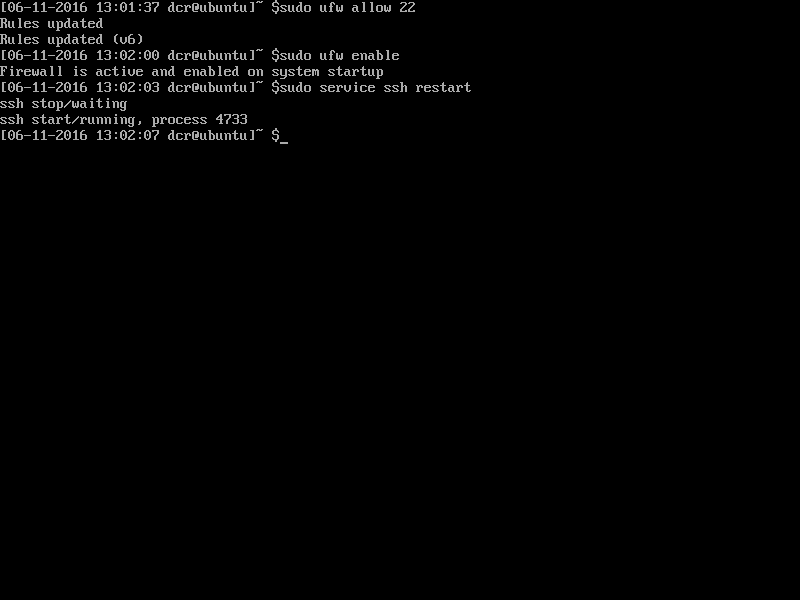
\includegraphics[scale=0.4]{ufw_ubu.png}
	\caption{Abrimos el puerto 22 en Ubuntu Server.}
\end{figure}

\subsection{¿Con qué comando puede abrir/cerrar un puerto usando firewall-cmd en CentOS? Muestre un ejemplo de cómo lo ha hecho.}
Con el comando sudo firewall-cmd --add-port=\verb|[nºpuerto]/| \verb|[tcp/udp]|. Además añadimos la opción --permanent para que el cambio quede activo en futuros reinicios del sistema. \cite{c3b}
\begin{figure}[H]
	\centering
	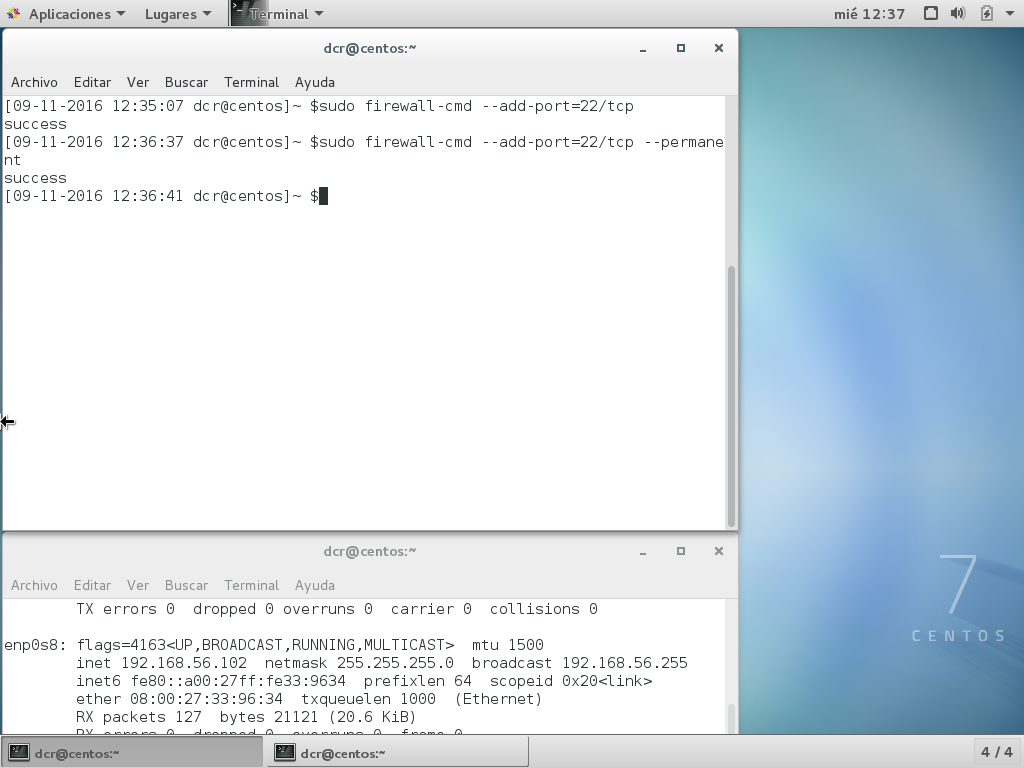
\includegraphics[scale=0.4]{fcmd.png}
	\caption{Abrimos el puerto 22 en CentOS.}
\end{figure}

\subsection{Utilice el comando nmap para ver que, efectivamente, los puertos están accesibles}
En nmap indicamos la dirección IP objetivo y podemos utilizar la opción -p para indicar el puerto o rango de puertos a buscar\cite{c3c}. Podemos obtener varios resultados (considerando una máquina externa, en mi caso, la máquina anfitriona), entre ellos: open (el puerto está abierto y un servicio está escuchando), close (el puerto está cerrado y no hay servicio escuchando) o filtered (el puerto está cerrado pero el servicio está escuchando).

\begin{figure}[H]
	\centering
	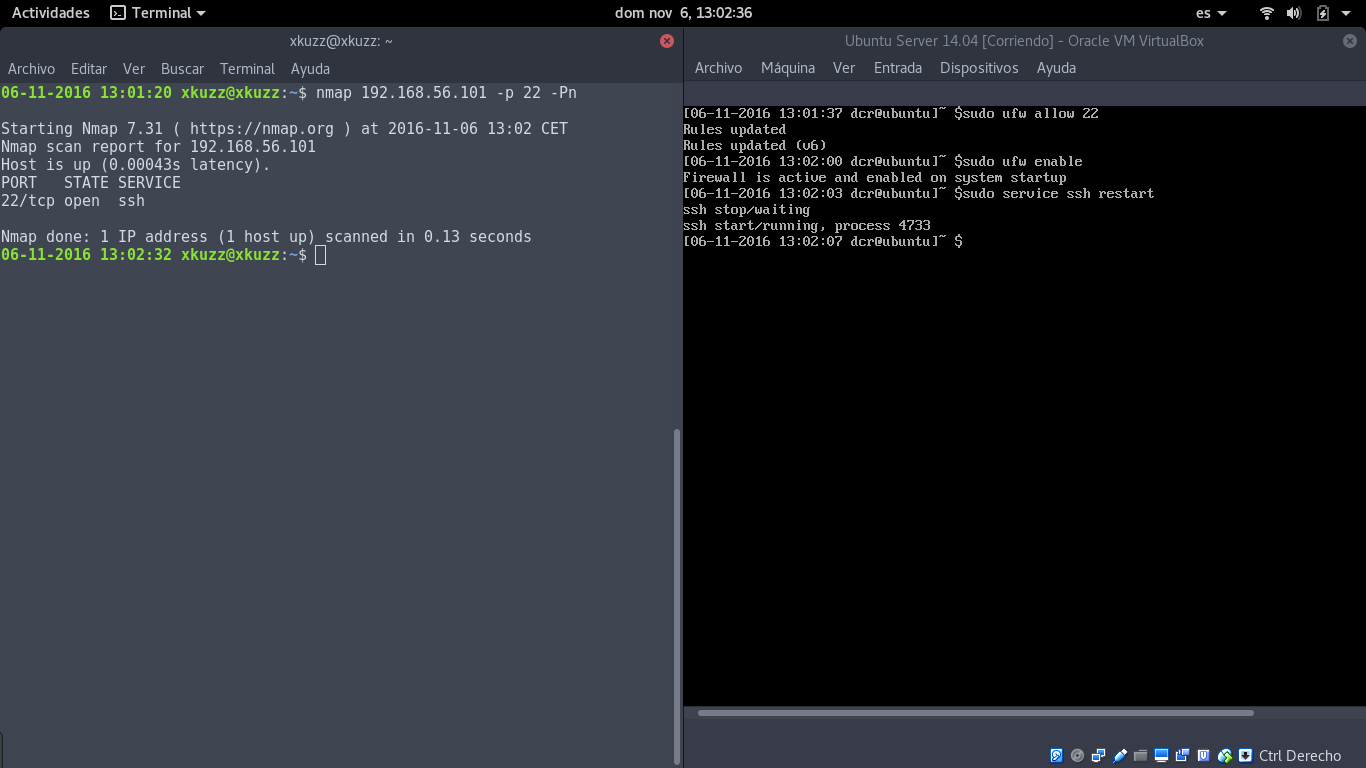
\includegraphics[scale=0.3]{nmap_ubu.png}
	\caption{Comprobamos desde el anfitrión que el puerto 22 está abierto en Ubuntu.}
\end{figure}

\begin{figure}[H]
	\centering
	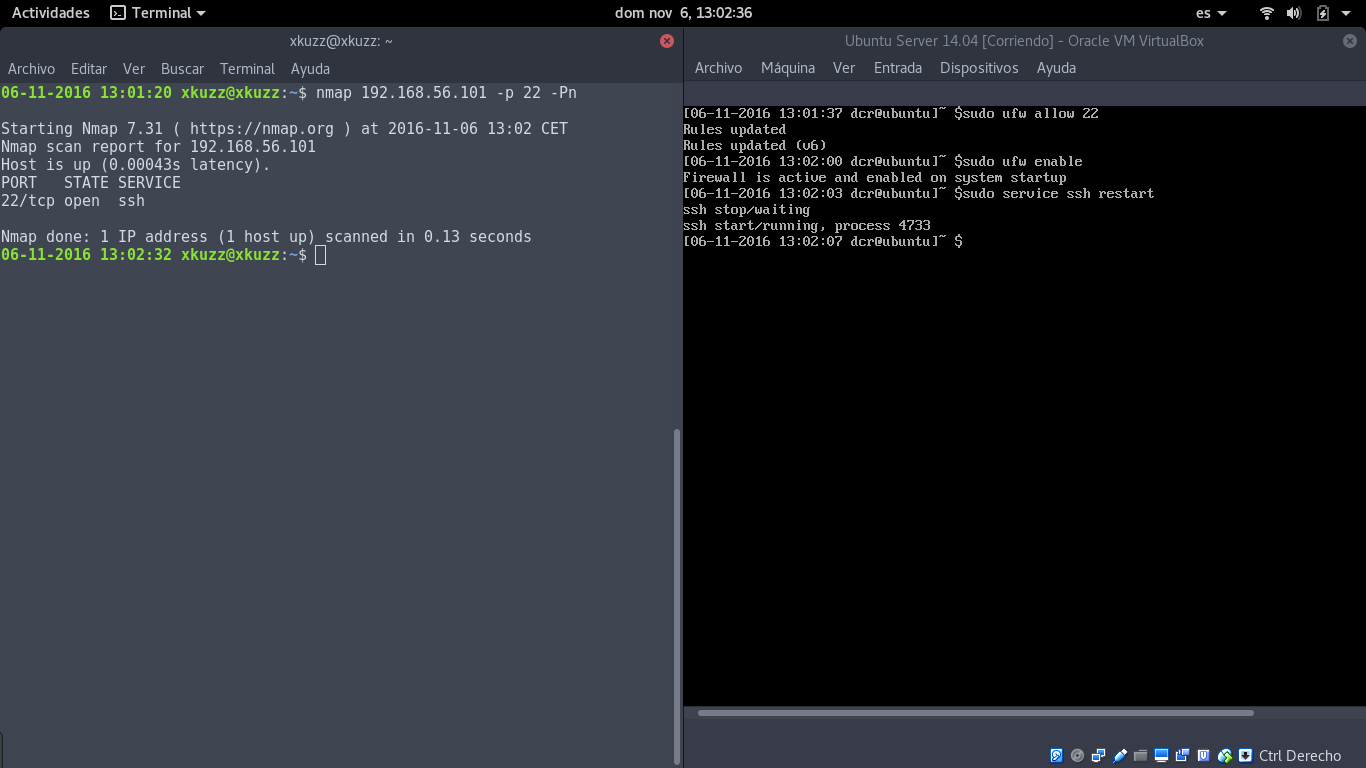
\includegraphics[scale=0.3]{nmap_ubu.png}
	\caption{Nmap desde el anfitrión antes y después de abrir el puerto en 22 en CentOS.}
\end{figure}
%----------------------------------------------------------------------------------------
%	Cuestión 4
%----------------------------------------------------------------------------------------
\section{¿Qué diferencia hay entre telnet y ssh?}
La principal diferencia entre ambos es que mientras que telnet es enviado como texto plano, ssh es encriptado. Por tanto, si alguien capturase una paquete telnet tendría acceso a la información que se estuviese transmitiendo e incluso si fuese en el momento de la autentificación tendría acceso a la contraseña introducida. Además, ssh utiliza firmas digitales para verificar la identidad de los extremos, por lo que ssh tampoco es directamente vulnerable con ataques de \textit{DNS Poisoning (conseguir que de un proveedor de DNS devuelva una IP modificada de un nombre de dominio)} o \textit{IP Spoofing (modificar la dirección IP origen de los paquetes de la capa de transporte del protocolo)}. \cite{c4}

%----------------------------------------------------------------------------------------
%	Cuestión 5
%----------------------------------------------------------------------------------------
\section{¿Para qué sirve la opción -X?  Ejecute remotamente, es decir, desde la máquina anfitriona (si tiene Linux) o desde la otra máquina virtual, el comando gedit en una sesión abierta con ssh. ¿Qué ocurre?}

\subsection{¿Para qué sirve la opción -X?}
Habilita el ``forwarding'' del servidor gráfico X11. Esto quiere decir que aunque la aplicación está siendo ejecutada en el máquina que actúa como servidor de ssh pero la interfaz gráfica se ejecuta en la máquina que actúa como cliente. \cite{c5a}

\subsection{Ejecute remotamente, es decir, desde la máquina anfitriona (si tiene Linux) o desde la otra máquina virtual, el comando gedit en una sesión abierta con ssh. ¿Qué ocurre?}
Si hubiésemos entrado a ssh sin el parámetro -X nos saldría el siguiente error al ejecutarlo.
\begin{figure}[H]
	\centering
	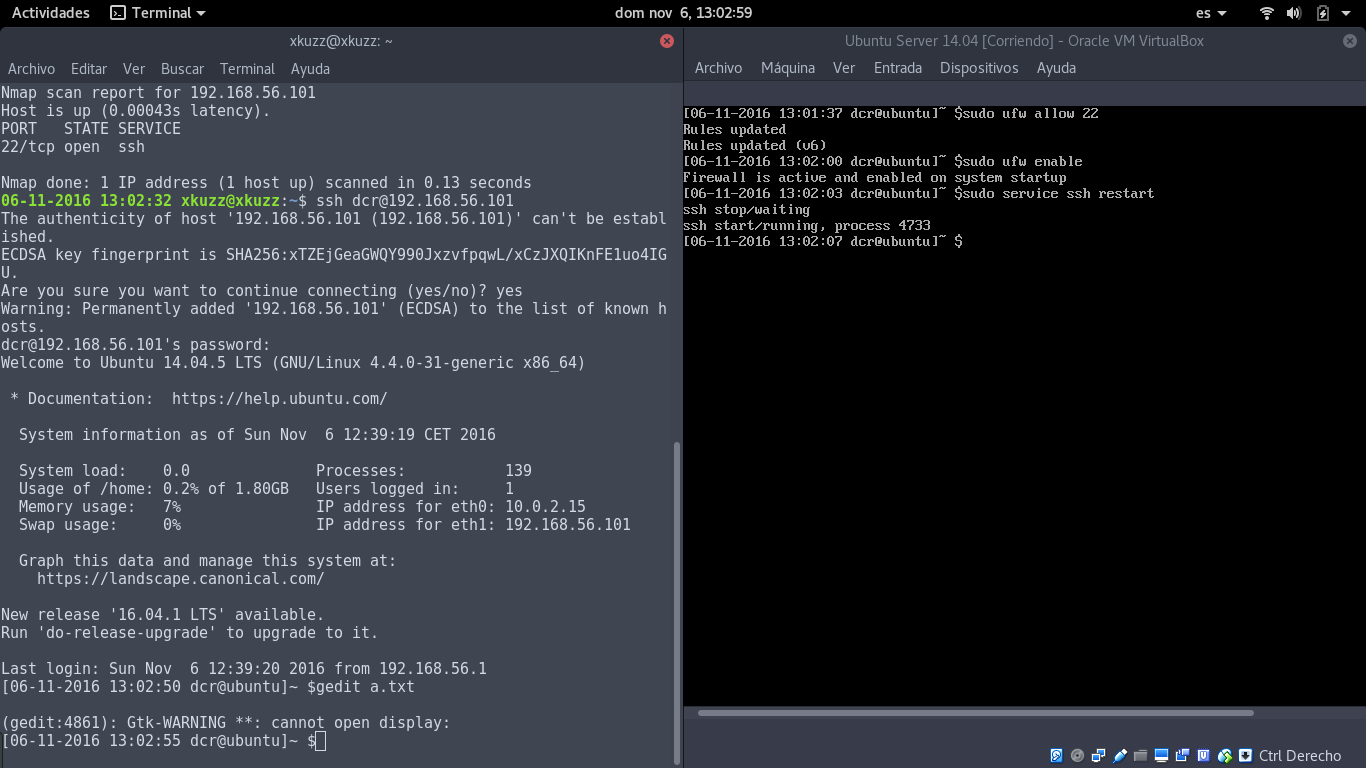
\includegraphics[scale=0.3]{gedit.png}
	\caption{Intentamos abrir gedit sin X11 forwading.}
\end{figure}

Al entrar con -X, el servidor gráfico se ejecuta del lado del cliente por lo que se nos abrirá una ventana con gedit, no obstante la modificación (como podemos comprobar en el cat realizado) se realiza en el servidor.
\begin{figure}[H]
	\centering
	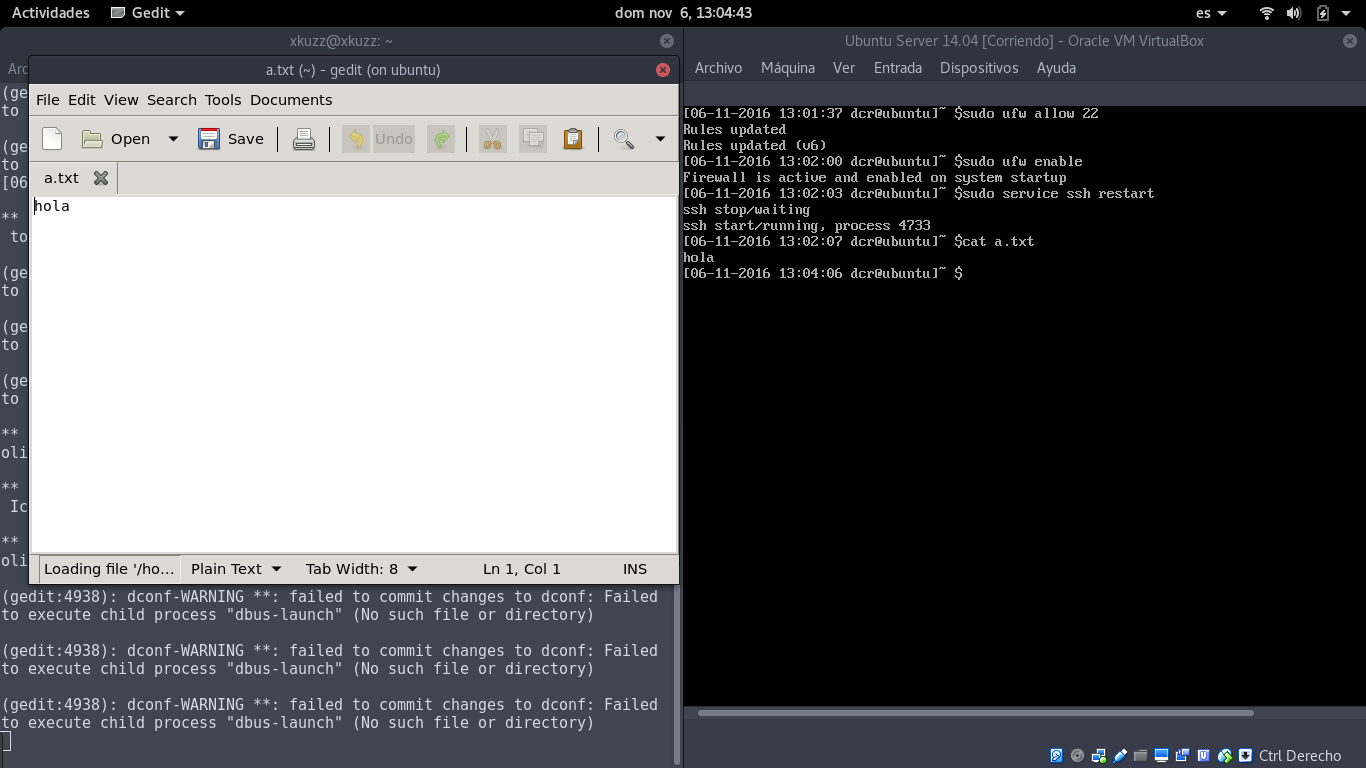
\includegraphics[scale=0.3]{geditX.png}
	\caption{Abrimos gedit con X11 forwarding.}
\end{figure}

%----------------------------------------------------------------------------------------
%	Cuestión 6
%----------------------------------------------------------------------------------------
\section{Muestre la secuencia de comandos y las modificaciones a los archivos para permitir acceder a la consola remota sin introducir la contraseña. Pruebe que funciona}
Para crear un nuevo par de llaves utilizamos el comando ssh-keygen \cite{c6a}. El comando nos pedirá la ubicación en la que guardar los archivos y una contraseña para la llave. Utilizamos la ubicación por defecto \verb|(~/.ssh/id_rsa)| y dejamos la contraseña en blanco para no tener que escribir nada pulsando Enter. Haciendo ls en el directorio \verb|~/.ssh| podemos observar a nuestra llave privada sólo puede acceder root con permisos de escritura y lectura, mientras que nuestra llave pública puede ser leída por todos pero sólo escrita por root.

\begin{figure}[H]
	\centering
	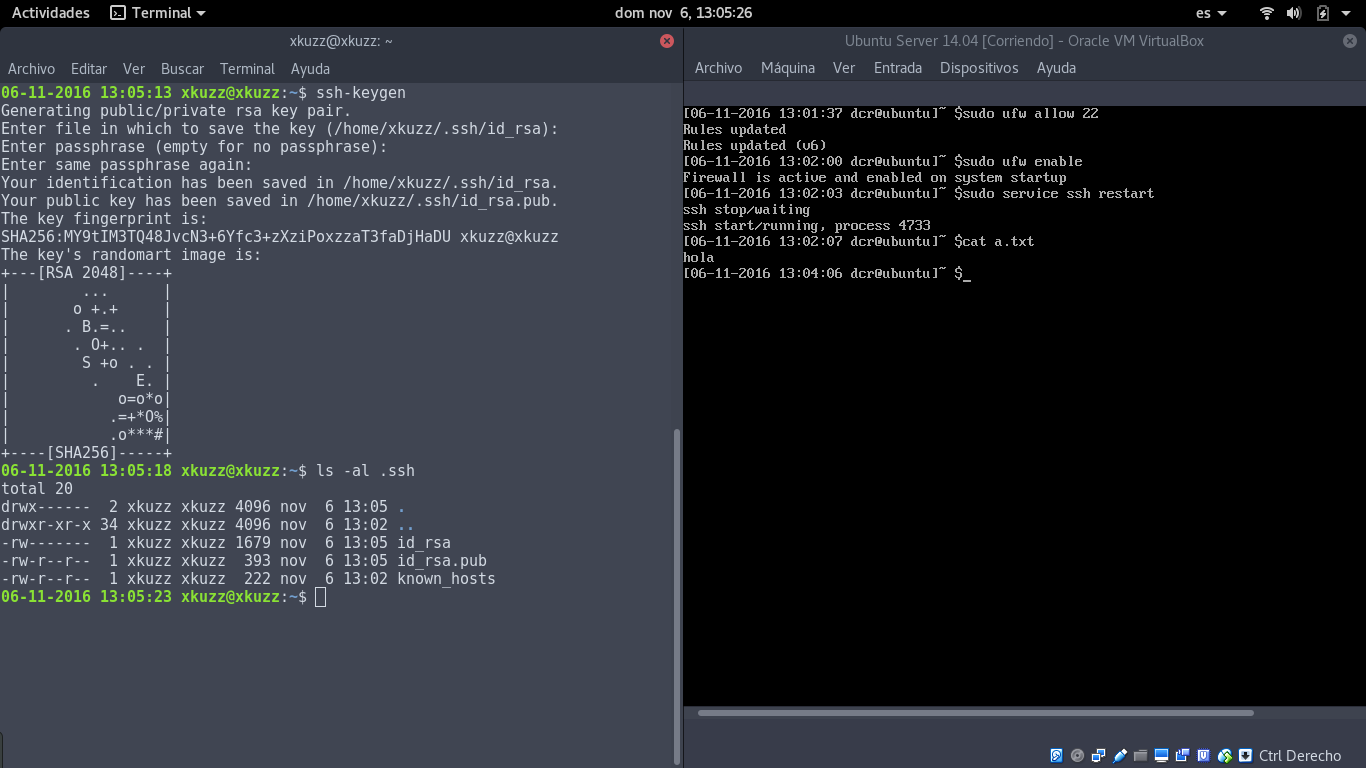
\includegraphics[scale=0.3]{ssh-keygen.png}
	\caption{Generación de la llave con ssh-keygen y comprobación de los permisos.}
\end{figure}

\textit{Nota: si nunca has usado una identidad en la máquina es posible que necesites ejecutar ssh-add\cite{c6b} para que la identidad sea añadida al agente de ssh. Ejecutar ssh-add añade las identidades de la ubicación por defecto de ssh-keygen} \linebreak

Para añadir nuestra llave al servidor y utilizarla como proveedor de identidad nuestro en el mismo utilizamos ssh-copy-id\cite{c6c} \verb|[nombreusuario]@[direccionIPservidor]|.
Una vez lo hemos añadido podemos entrar sin necesidad de escribir la contraseña al servidor de ssh, tal y como podemos comprobar en el ejemplo.

\begin{figure}[H]
	\centering
	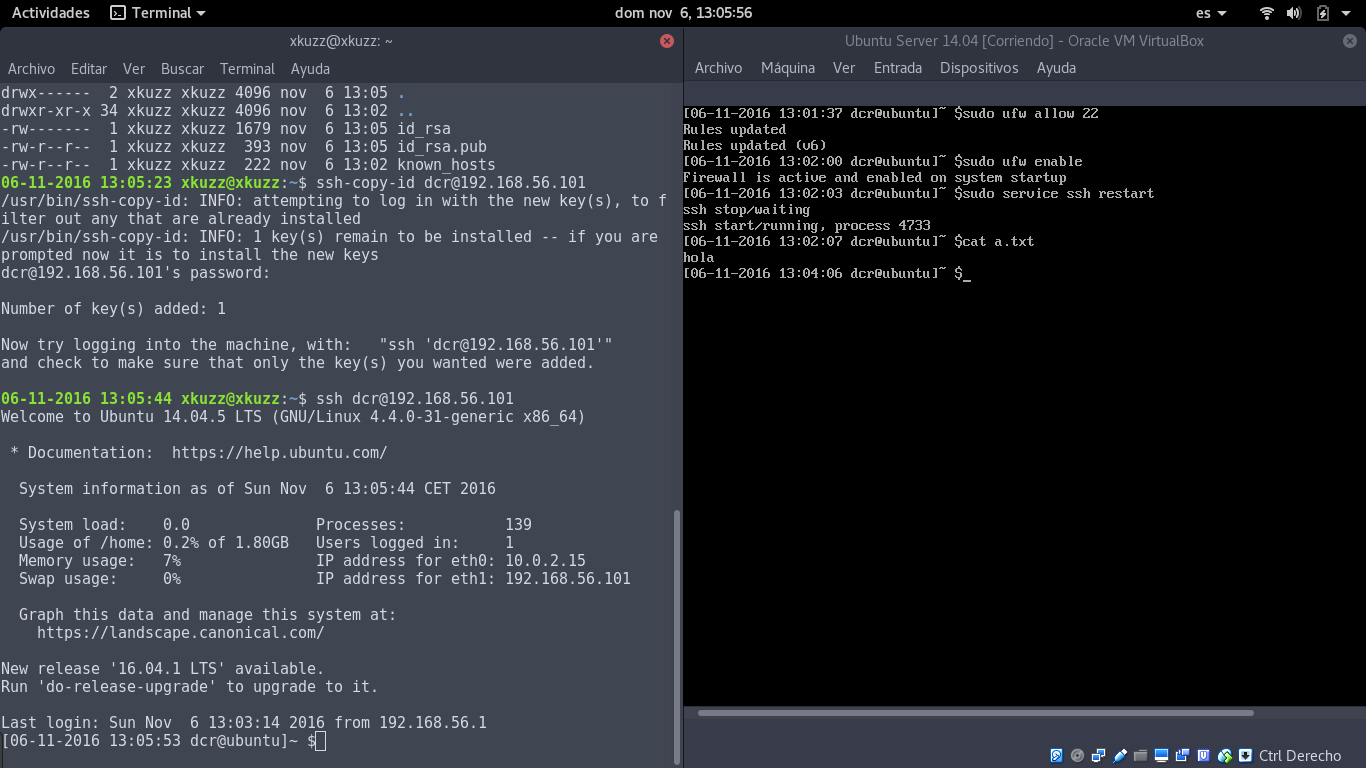
\includegraphics[scale=0.3]{ssh-copy-id.png}
	\caption{Añadimos la identidad en el servidor con ssh-copy-id y comprobamos que podemos acceder sin contraseña.}
\end{figure}

%----------------------------------------------------------------------------------------
%	Cuestión 7
%----------------------------------------------------------------------------------------
\section{¿Qué archivo es el contiene la configuración del servicio ssh? ¿Qué parámetro hay que modificar para evitar que el usuario root acceda?Cambie el puerto por defecto y compruebe que puede acceder.}
El archivo es \verb|/etc/ssh/sshd_config|. \cite{c7a} \linebreak
Para evitar que root pueda acceder debemos de poner el parámetro PermitRootLogin a no. \cite{c7b} Por defecto, en Ubuntu, por la configuración inicial del servicio, el parámetro esta puesto a without-password, eso quiere decir que no nos permite entrar a no ser que tengamos una llave asociada al usuario. Vemos que al probarlo nos pide contraseña pero no la da por válida.
\begin{figure}[H]
	\centering
	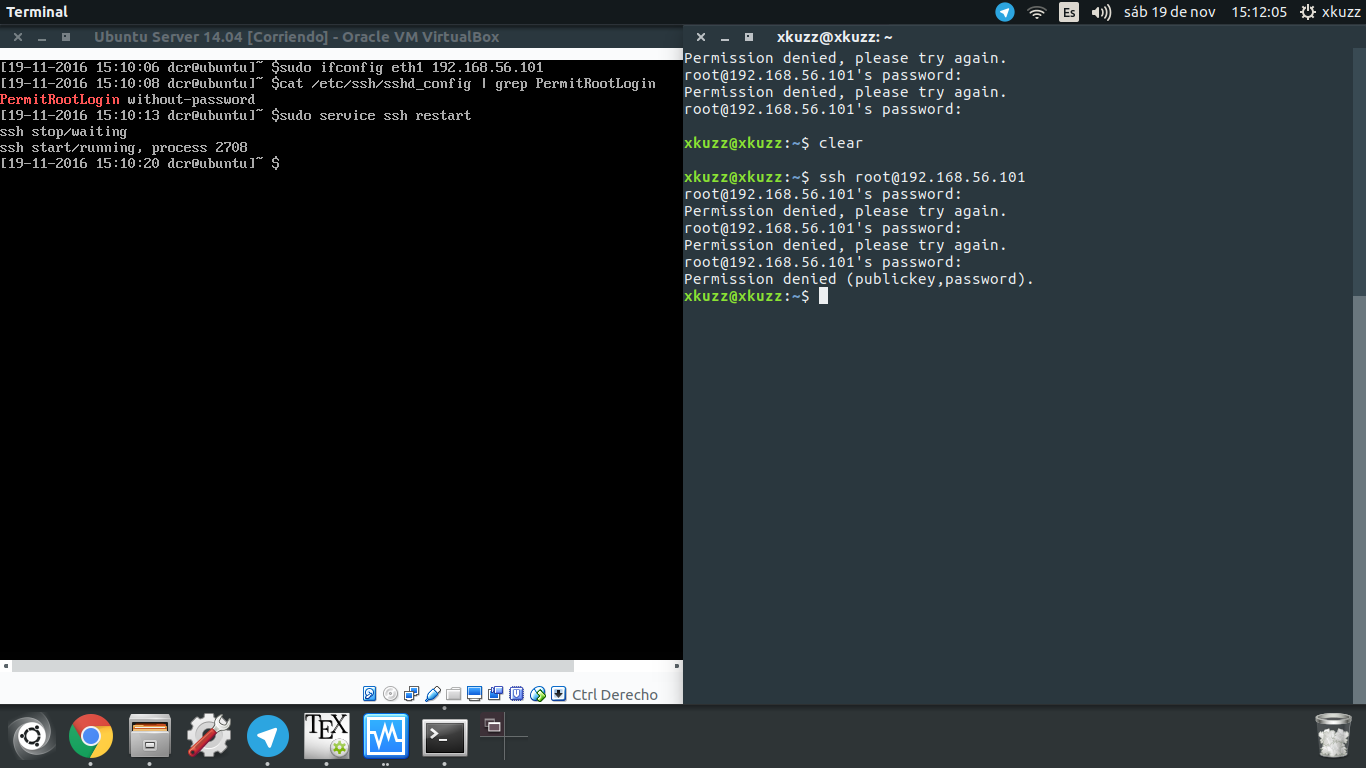
\includegraphics[scale=0.3]{rootwp.png}
	\caption{Intentamos acceder a ssh con el parámetro without-password.}
\end{figure}

Tras poner una contraseña al usuario root con passwd (en Ubuntu, por defecto, root no tiene la contraseña configurada) y poner el parámetro a yes vemos que podemos acceder a ssh.

\begin{figure}[H]
	\centering
	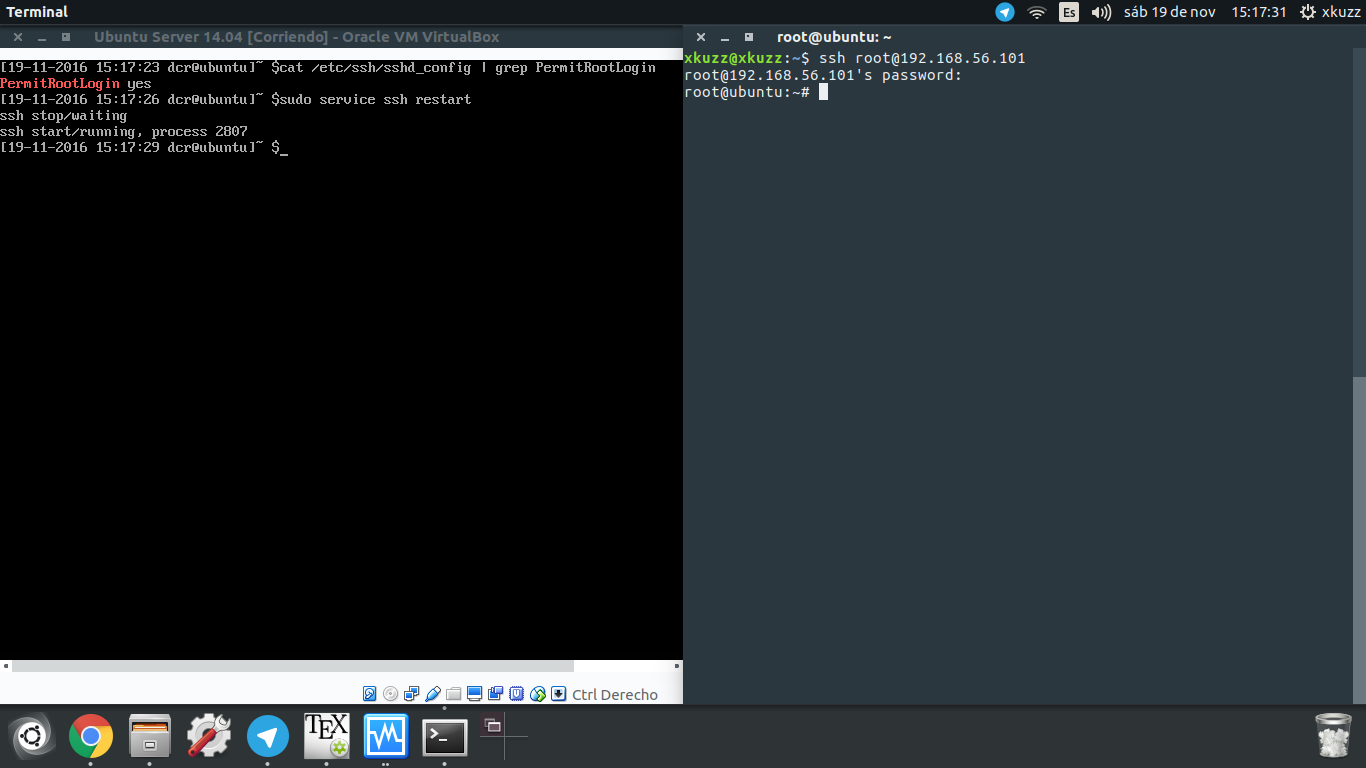
\includegraphics[scale=0.3]{rootyes.png}
	\caption{Intentamos acceder a ssh con el parámetro yes.}
\end{figure}

Por último, comprobemos que no nos deja acceder con el parámetro a no.
\begin{figure}[H]
	\centering
	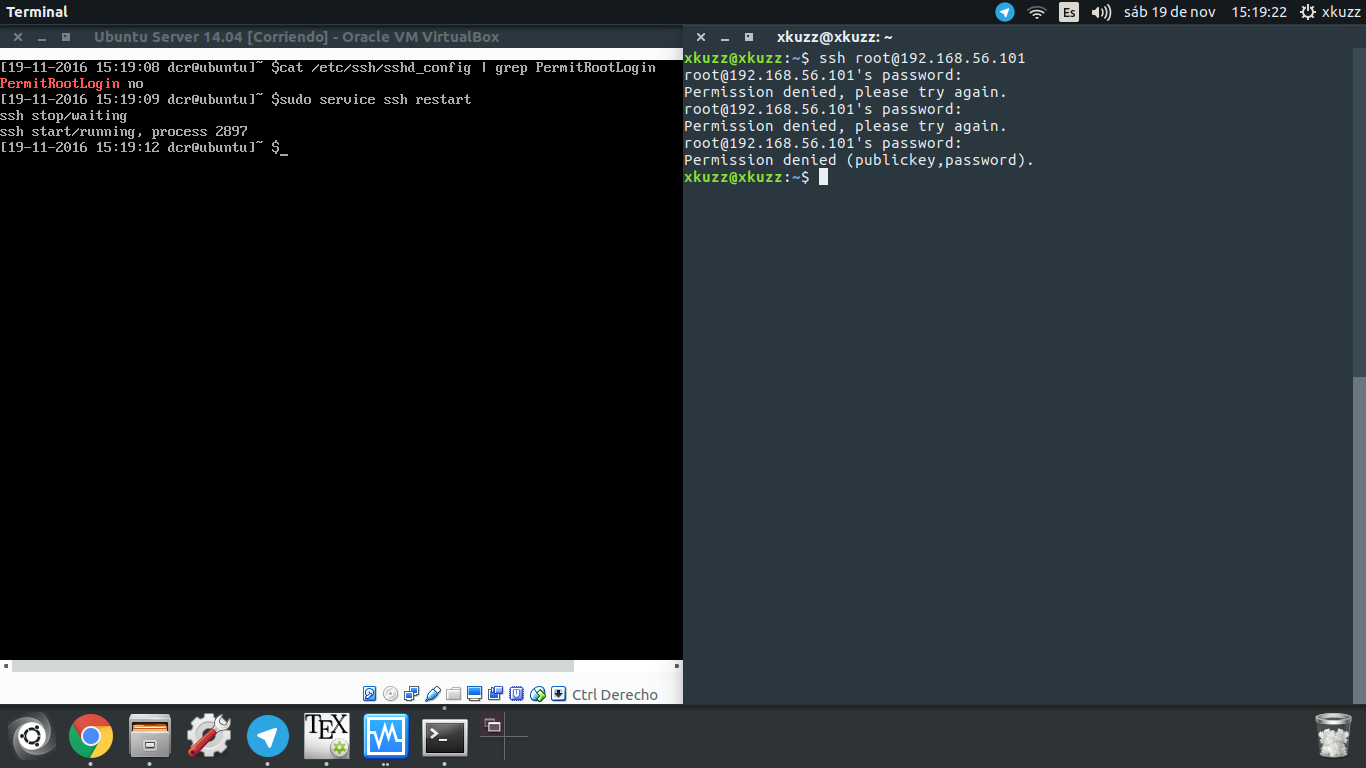
\includegraphics[scale=0.3]{rootno.png}
	\caption{Intentamos acceder a ssh con el parámetro no.}
\end{figure}


Cambiamos en el puerto por defecto en el parámetro Port de \verb|/etc/ssh/sshd_config|, activamos el puerto en el firewall y, al intentarlo, vemos que no podemos entrar (es necesario reiniciar el servicio).
\begin{figure}[H]
	\centering
	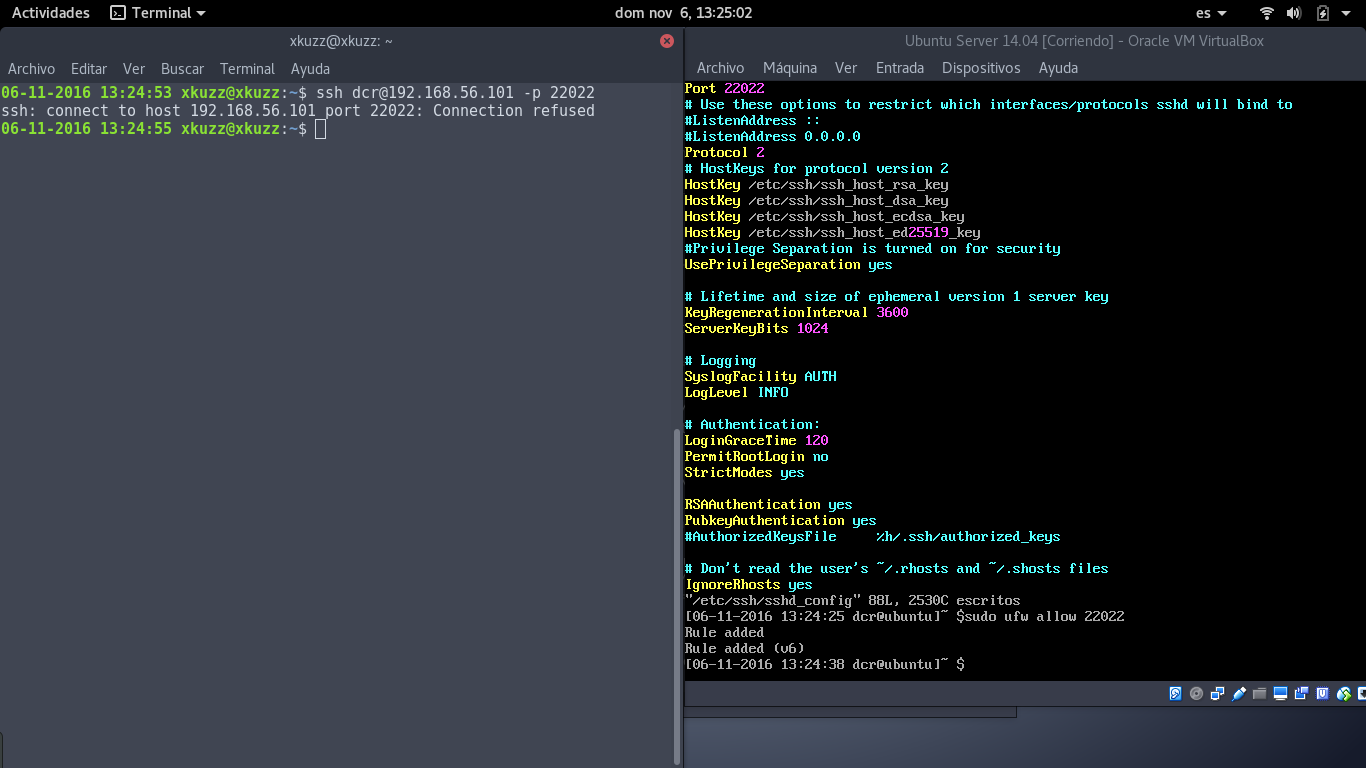
\includegraphics[scale=0.3]{servicioSinReiniciar.png}
	\caption{Intentamos acceder a ssh tras modificar el puerto y abrirlo en el firewall.}
\end{figure}

%----------------------------------------------------------------------------------------
%	Cuestión 8
%----------------------------------------------------------------------------------------
\section{Indique si es necesario reiniciar el servicio. ¿Cómo se reinicia un servicio en Ubuntu?, ¿y en CentOS? Muestre la secuencia de comandos para hacerlo.}
Como hemos podido comprobar en la pregunta anterior sí es necesario reiniciar el servicio.\linebreak
 En Ubuntu podemos utilizar (necesitas permisos de administrador) \verb| service ssh restart|\cite{c8a}.\linebreak
 En CentOS podemos utilizar (necesitamos permisos de administrador) \verb| systemctl restart sshd |\cite{c8b}. \linebreak
 Así podemos comprobar siguiendo el ejemplo del ejercicio anterior, que tras reiniciar podemos a acceder a ssh desde el nuevo puerto.
 \begin{figure}[H]
	\centering
	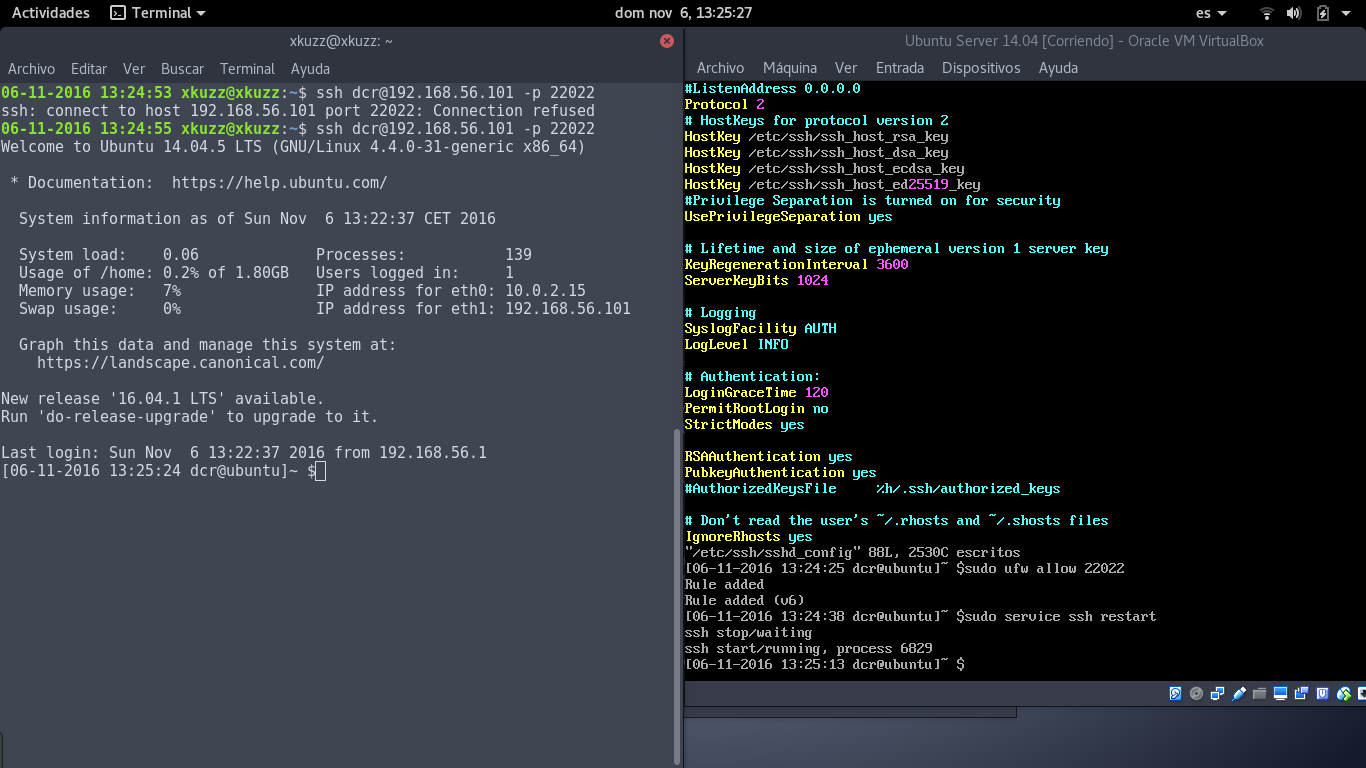
\includegraphics[scale=0.3]{servicioReiniciado.png}
	\caption{Accedemos a ssh tras reiniciar el servicio.}
\end{figure}

%----------------------------------------------------------------------------------------
%	Cuestión 9
%----------------------------------------------------------------------------------------
\section{Muestre los comandos que ha utilizado para instalar LAMP en Ubuntu Server y en CentOS (aunque en este último puede utilizar la GUI, en tal caso, realice capturas de pantalla). Compruebe que la instalación ha sido correcta.}
Para instalarlo en Ubuntu utilizamos el comando (con permisos de administrador) tasksel install lamp-server. \cite{c9a}

Durante la instalación se nos solicitará que escojamos la contraseña de root para nuestro servidor MySQL que en este caso he vuelto a poner como \verb|practicas,ISE|. \linebreak

Una vez instalado, para poder comprobar su funcionamiento, debemos abrir los puertos 80 (HTTP) y 443 (HTTPS).

\begin{figure}[H]
	\centering
	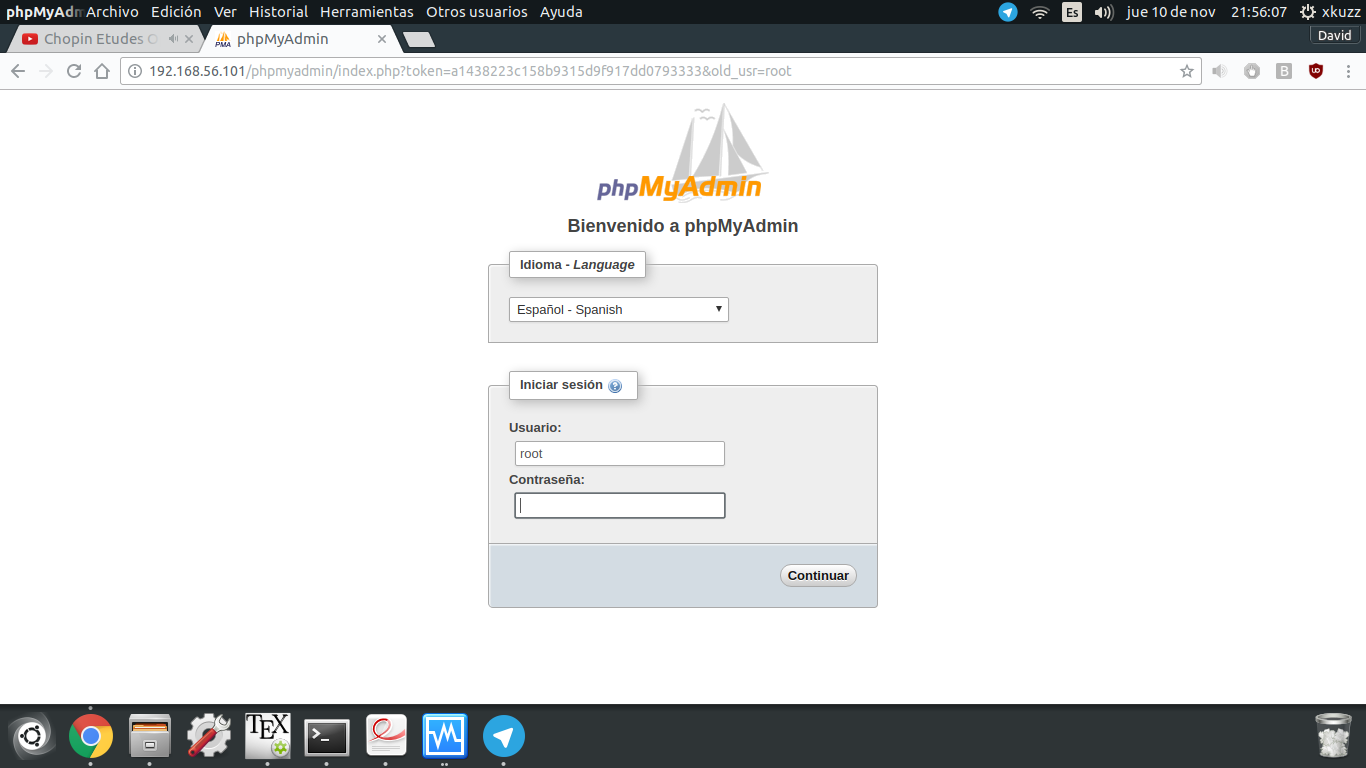
\includegraphics[scale=0.3]{phpmyadmin1.png}
	\caption{Página de inicio de sesión de phpMyAdmin}
	\label{fig:phpmyadmin}
\end{figure}

Podemos comprobar que la instalación es correcta en Ubuntu accediendo a phpMyAdmin (instalado en la cuestión 13) ya que requiere tanto del servidor web apache, como de MySQL y de php.\linebreak

Para instalarlo en CentOS\cite{c9b} uso los siguientes comandos con permisos de administrador.
\begin{itemize}
\item yum install httpd httpd-manual \verb|\\| (Instalamos servidor HTTP)
\item firewall-cmd --permanent --add-service=http \verb|\\| (Abrimos puerto HTTP)
\item firewall-cmd --permanent --add-service=https \verb|\\| (Abrimos puerto HTTPS)
\item yum install mariadb-server mariadb \verb|\\| (Instalamos MariaDB, una bifurcación de MySQL)
\item systemctl start mariadb \verb|\\| (Iniciamos el servicio de MariaDB)
\item mysql\_secure\_installation \verb|\\| (Ejecutamos un script que nos permite entre otros cambiar la contraseña del usuario root en MariaDB, el resto de opciones han sido dejadas al valor por defecto presionando 'Enter')
\item sytemctl enable mariadb \verb|\\| (Iniciamos el servicio de MariaDB al arrancar el sistema)
\item yum install php php-mysql \verb|\\| (Instalamos php y el módulo de MySQL para php)
\item systemctl restart httpd \verb|\\| (Reiniciamos el servidor web)
\end{itemize}

Por cambiar, vamos a probar que funciona correctamente en CentOS creando el archivo /var/www/html/index.php el que vemos a la derecha en la siguiente figura (en el que utilizamos \verb|mysql_connect(...)|\cite{c9c} para conectarnos a MySQL y \verb|phpinfo()|\cite{c9d} para ver la información de php del servidor.

\begin{figure}[H]
	\centering
	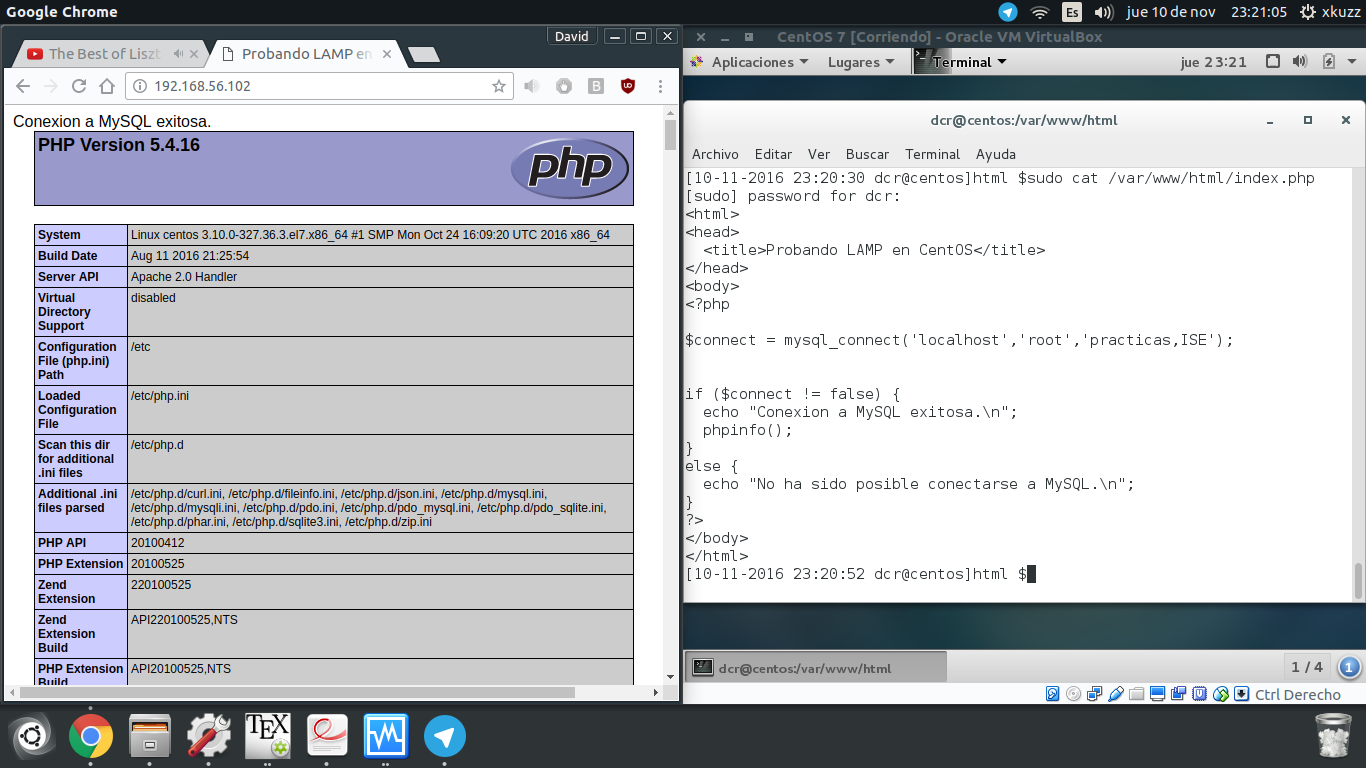
\includegraphics[scale=0.3]{lampTest.png}
	\caption{A la izquierda probamos desde la máquina anfitrión que LAMP está completamente operativo. A la derecha el código utilizado para dicha comprobación.}
\end{figure}





%----------------------------------------------------------------------------------------
%	Cuestión 10
%----------------------------------------------------------------------------------------
\section{Realice la instalación de IIS usando GUI o PowerShell y compruebe que el servicio está funcionando accediendo a la MV a través de la anfitriona.}
Vamos a instalar según nos indican en la página de IIS \cite{c10} mediante la GUI y escogiendo las características previamente nombradas. Primero abrimos el Administrador del servidor.

\begin{figure}[H]
	\centering
	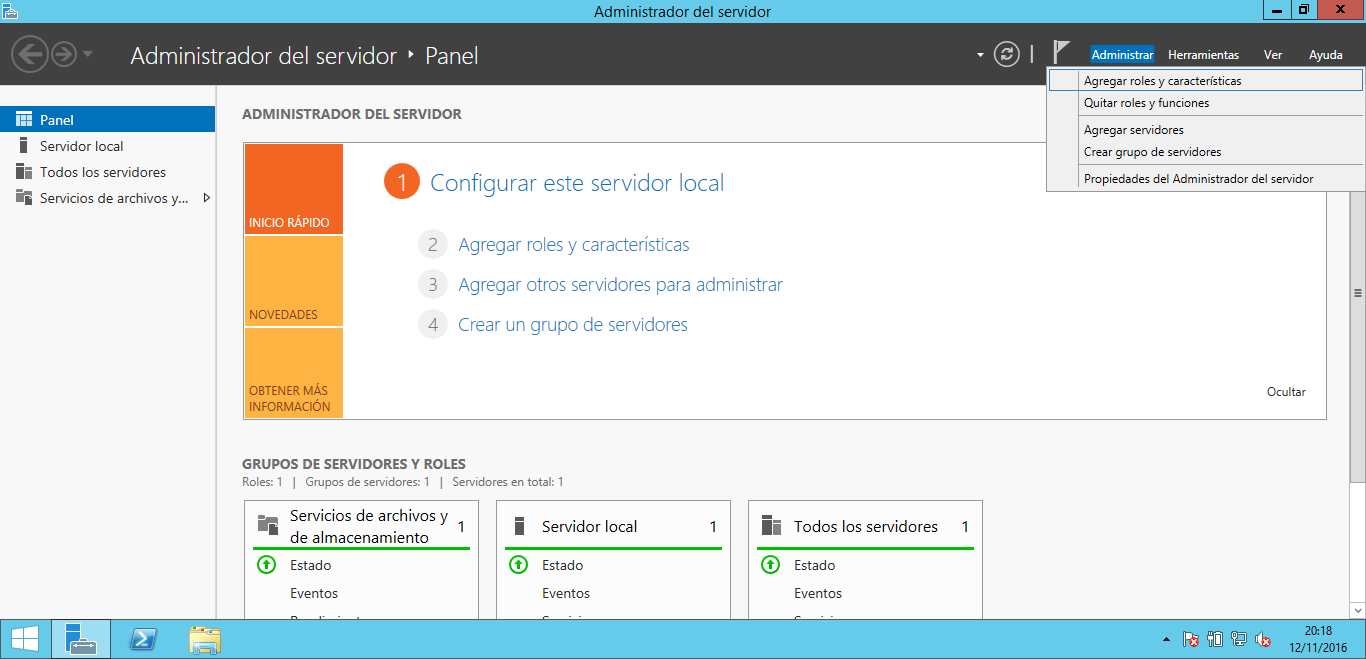
\includegraphics[scale=0.4]{iis1.png}
	\caption{Hacemos click en administración > Agregar roles y características}
\end{figure}

\begin{figure}[H]
	\centering
	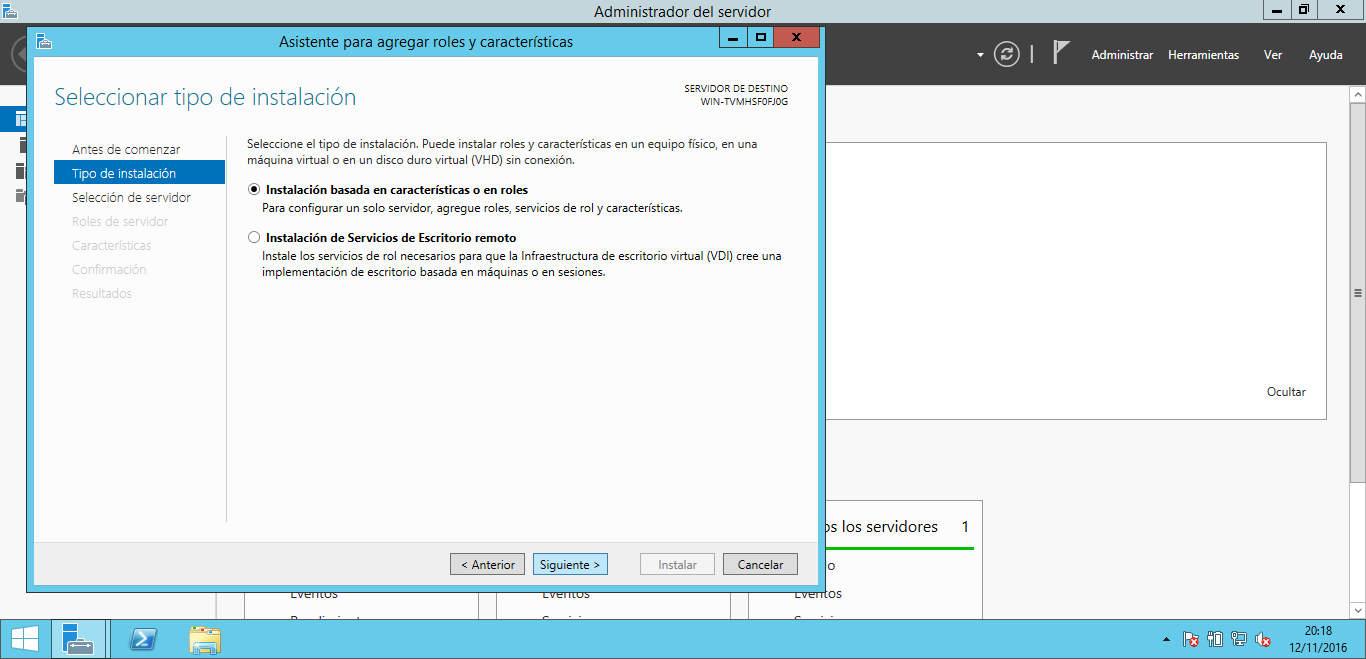
\includegraphics[scale=0.4]{iis2.png}
	\caption{Dejamos instalación basada en característica y/o roles y pulsamos Siguiente.}
\end{figure}

\begin{figure}[H]
	\centering
	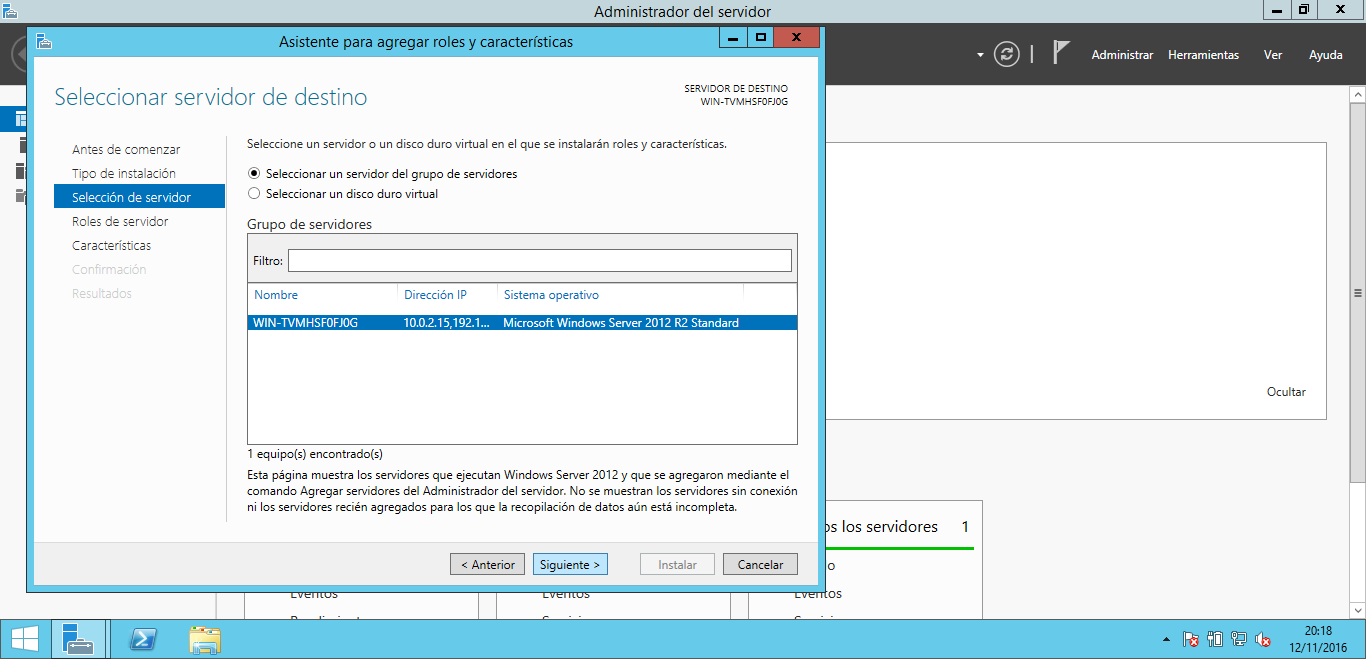
\includegraphics[scale=0.4]{iis3.png}
	\caption{Dejamos seleccionado el único servidor del grupo de servidores y pulsamos Siguiente.}
\end{figure}

\begin{figure}[H]
	\centering
	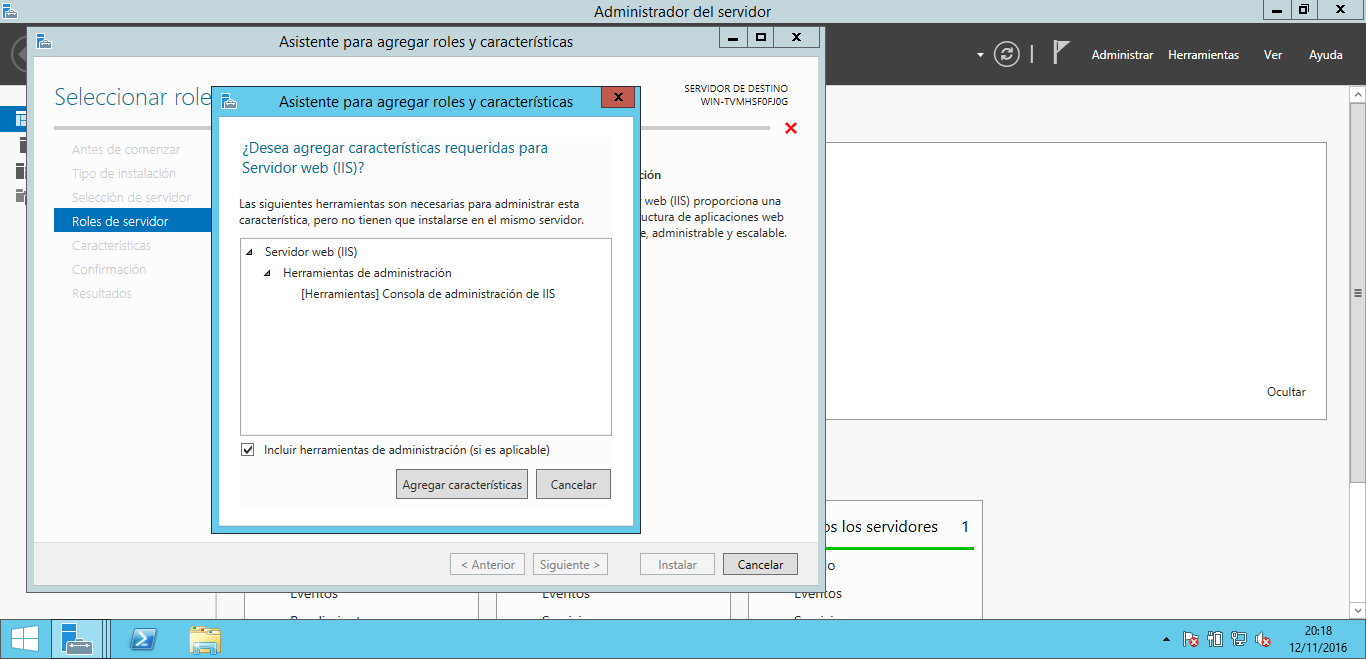
\includegraphics[scale=0.4]{iis4.png}
	\caption{Marcamos IIS y nos saldrá una ventana por si queremos instalar herramientas de administración. Dejamos
	marcado que sí y pulsamos Agregar Características}
\end{figure}

\begin{figure}[H]
	\centering
	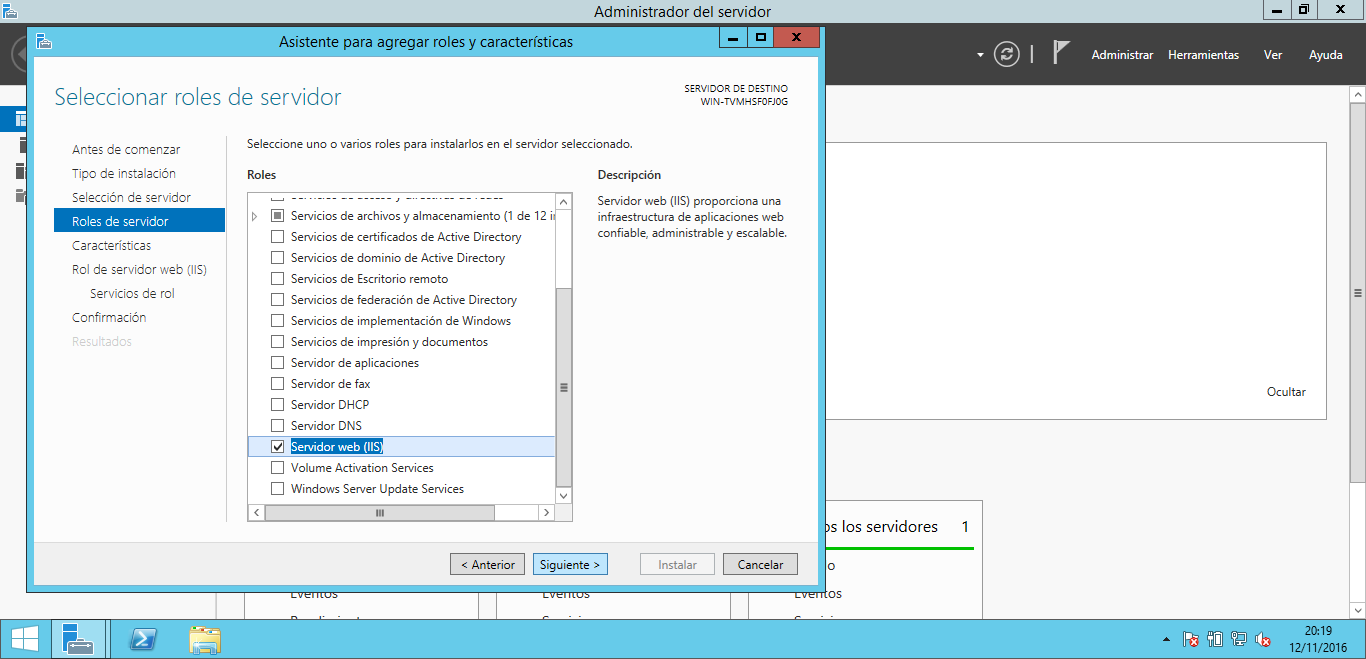
\includegraphics[scale=0.4]{iis5.png}
	\caption{Con IIS previamente marcado y tras Agregar Características pulsamos Siguientes.}
\end{figure}

\begin{figure}[H]
	\centering
	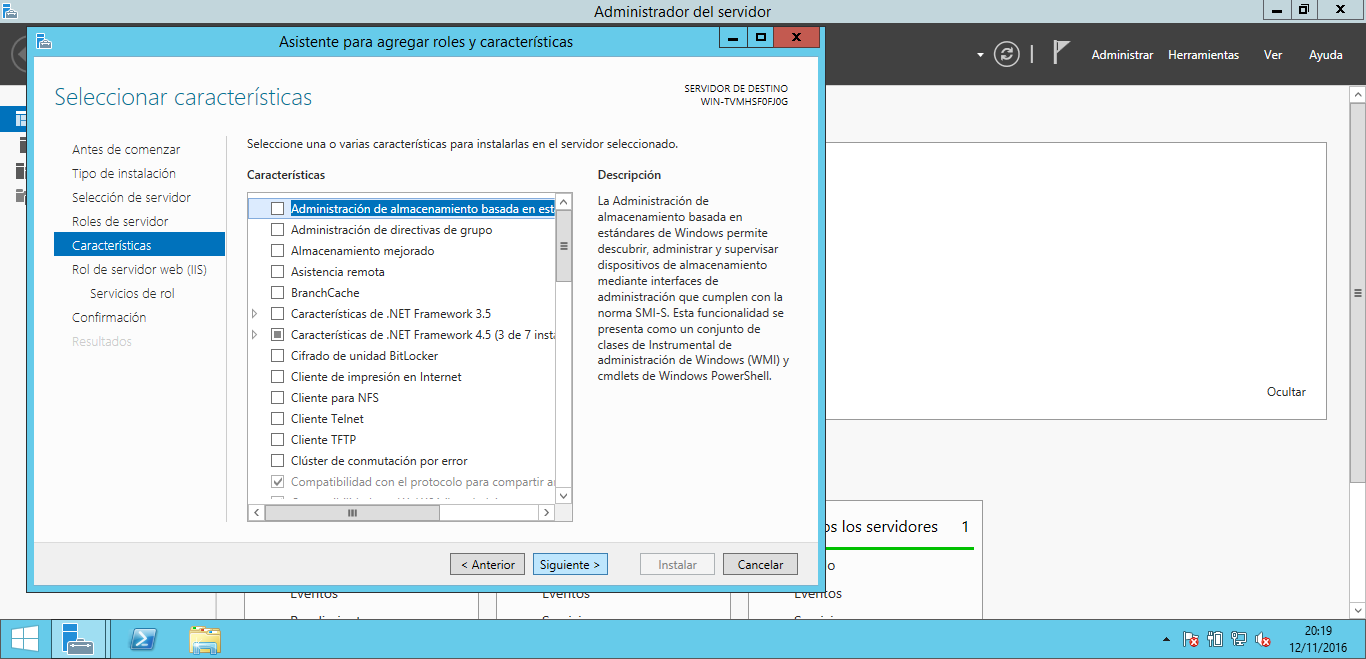
\includegraphics[scale=0.4]{iis6.png}
	\caption{En el menú de características pulsamos Siguiente.}
\end{figure}

\begin{figure}[H]
	\centering
	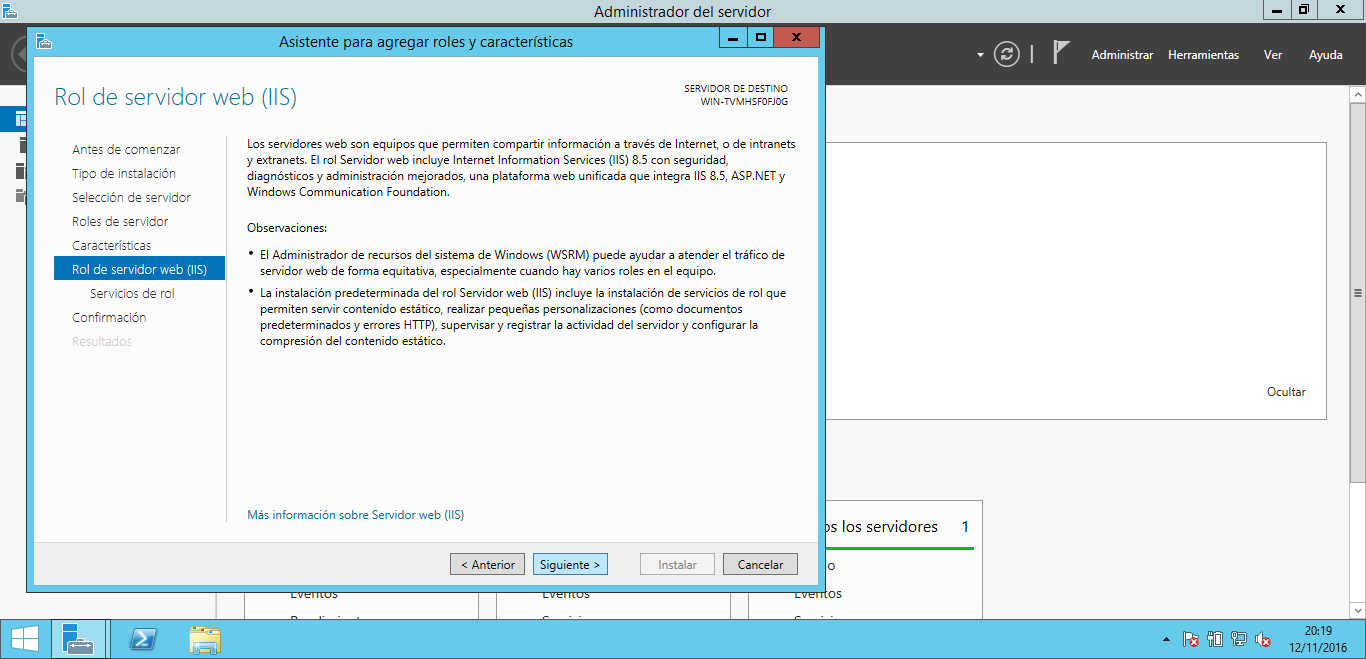
\includegraphics[scale=0.4]{iis7.png}
	\caption{Volvemos a pulsar Siguiente}
\end{figure}

\begin{figure}[H]
	\centering
	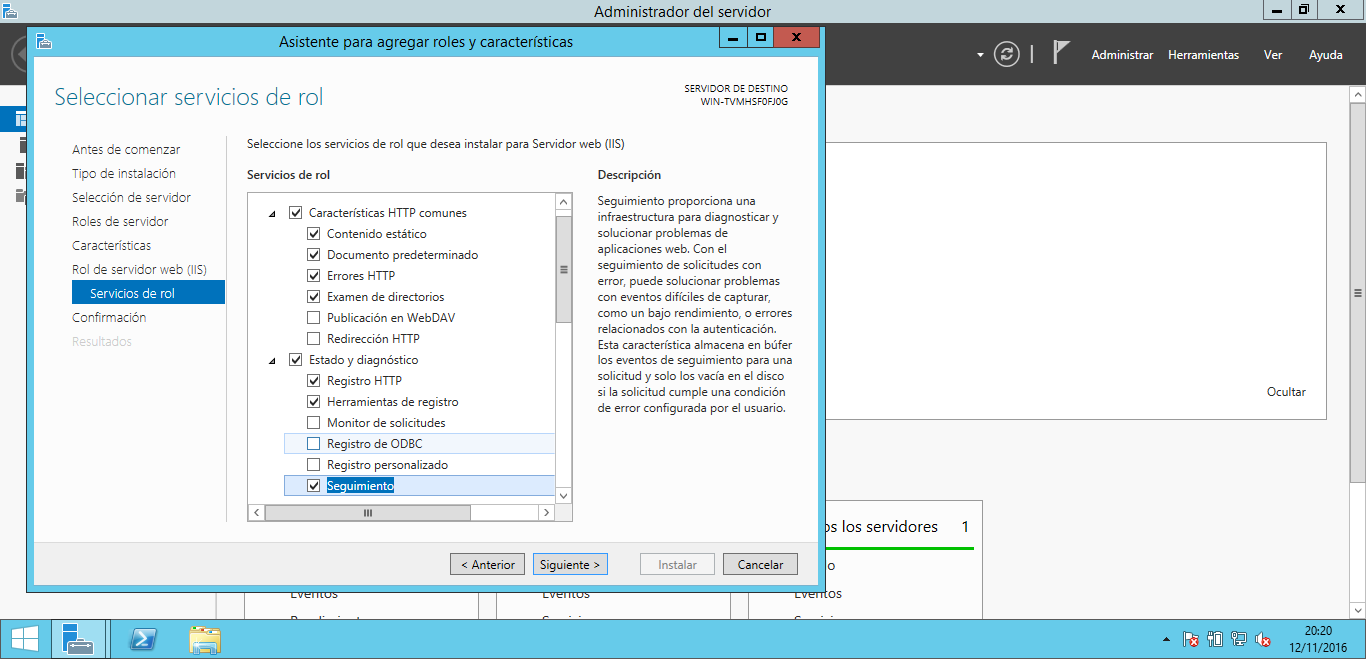
\includegraphics[scale=0.4]{iis8.png}
	\caption{Aparte de las opciones ya marcadas marcamos Herramientas de registro y Seguimiento.}
\end{figure}

\begin{figure}[H]
	\centering
	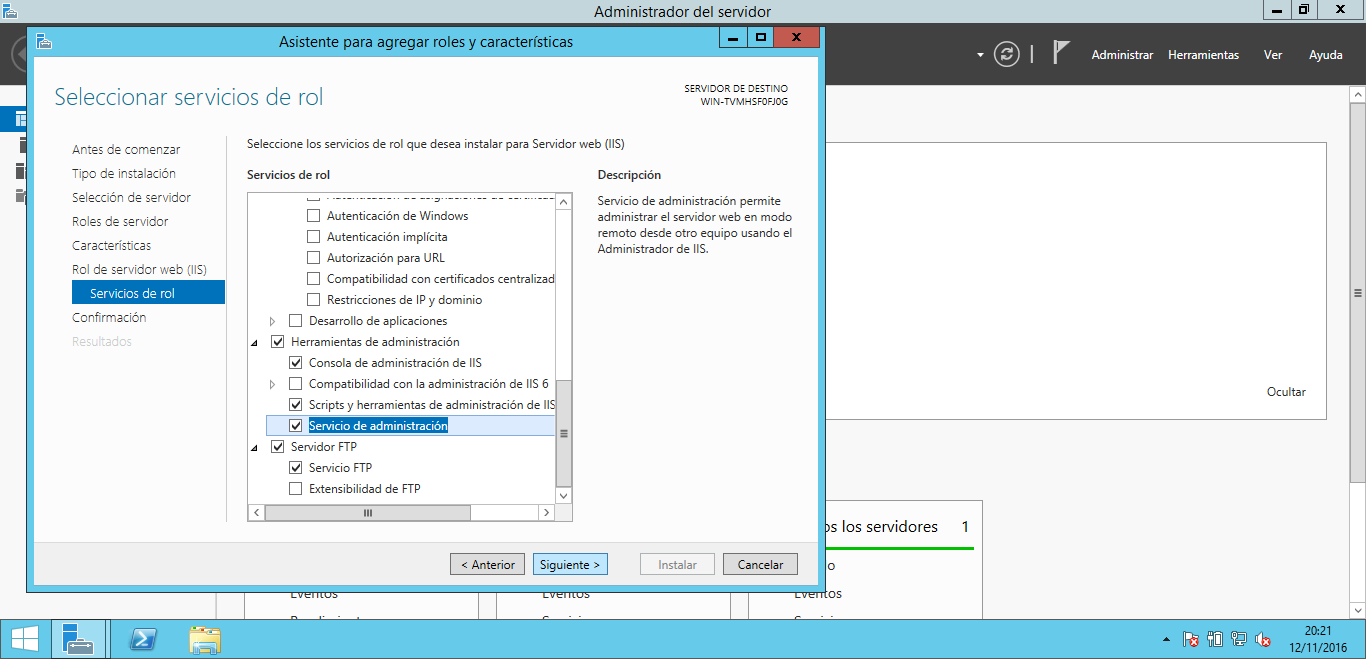
\includegraphics[scale=0.4]{iis9.png}
	\caption{Aparte de las opciones ya marcadas marcamos: Scripts y herramientas de administración de IIS, Servicio de
	administración, Servidor FTP y Servicio FTP. }
\end{figure}

\begin{figure}[H]
	\centering
	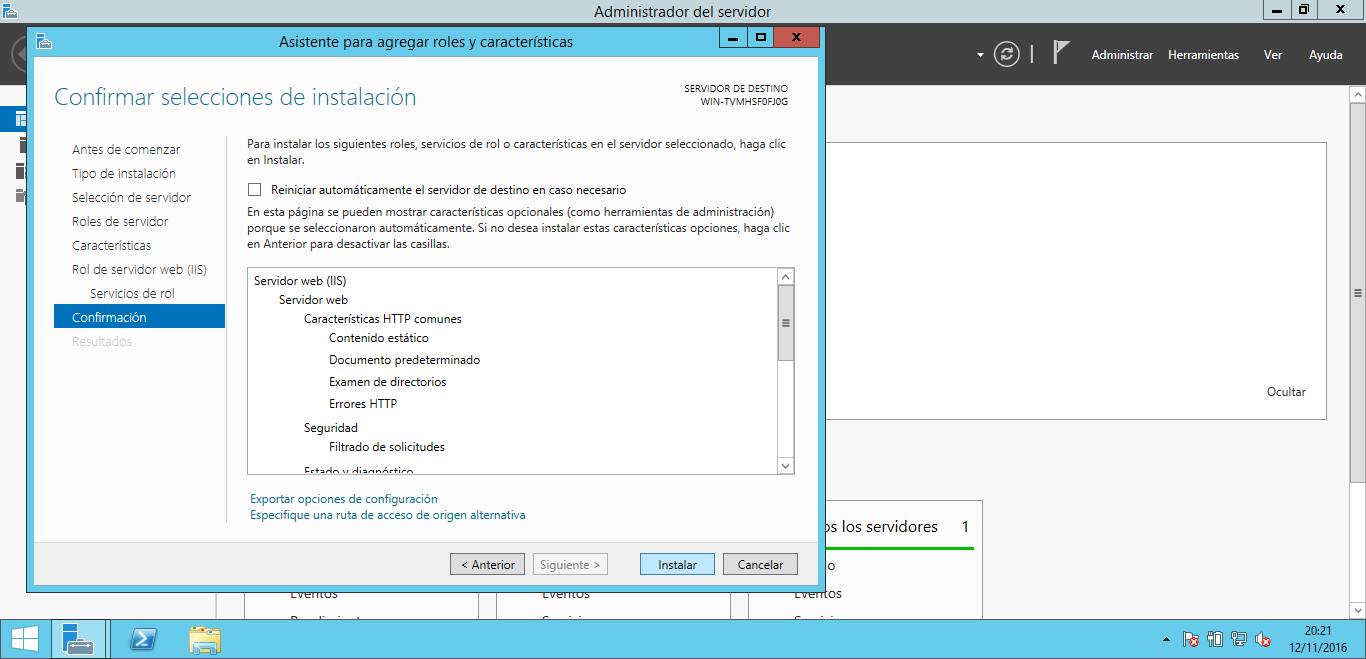
\includegraphics[scale=0.4]{iis10.png}
	\caption{Se nos ofrece un resumen en el que podemos comprobar que todo es correcto y pulsamos en Instalar.}
\end{figure}


Tras acabar el proceso de instalación probamos a entrar desde la máquina anfitriona viendo lo siguiente:
\begin{figure}[H]
	\centering
	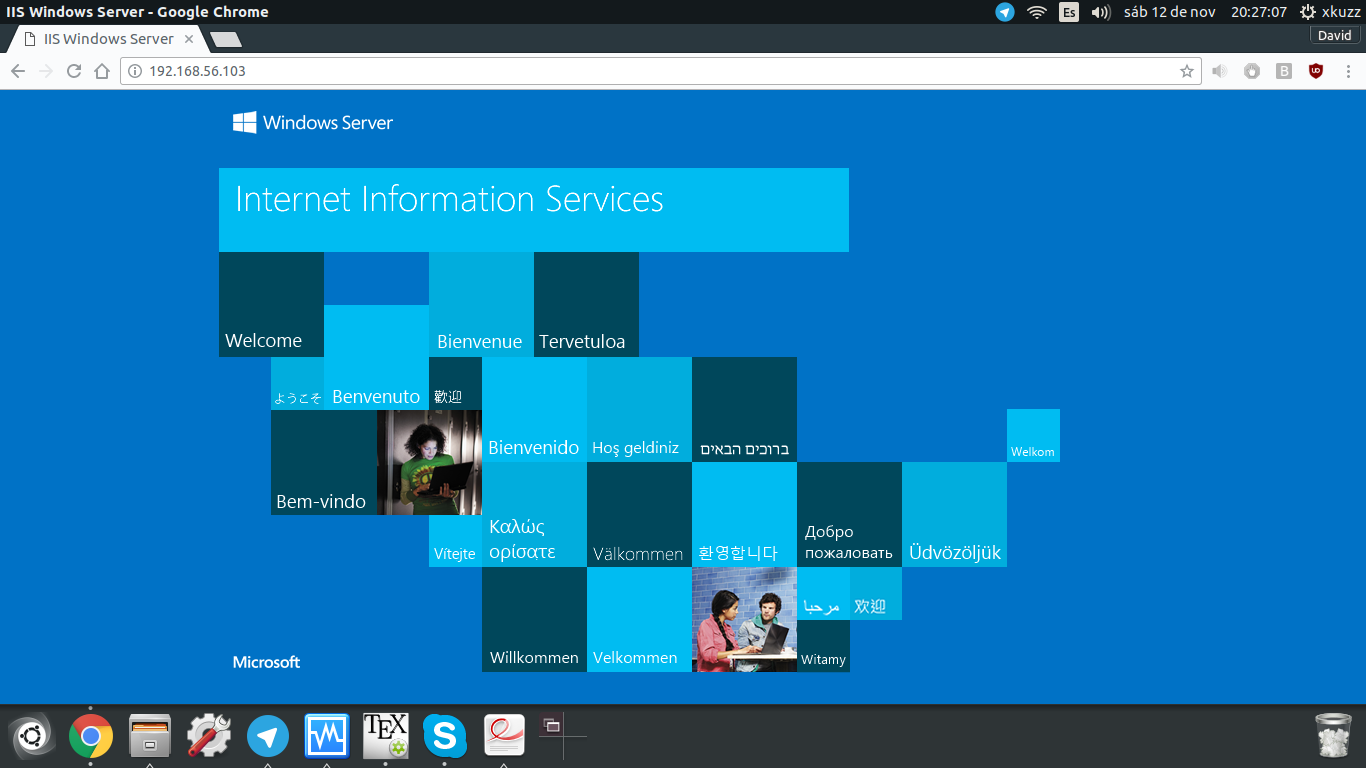
\includegraphics[scale=0.3]{iisTest.png}
	\caption{Probamos que IIS desde la máquina anfitriona.}
\end{figure}


%----------------------------------------------------------------------------------------
%	Cuestión 11
%----------------------------------------------------------------------------------------
\section{Muestre un ejemplo de uso del comando patch.}
Patch \cite{c11} nos permite modificar un archivo a partir de una versión diferente. Vamos a mostrar un ejemplo de su uso con el siguiente programa escrito en C++11.

\begin{verbatim}
#include <iostream>
#include <vector>
int main () {
  std::vector<int> numeros {2, 6, 10, 15, 32, 99};
  for (auto a: numeros) 
    std::cout << "Al sumar 2 a " << a << " obtenemos " << a + 1 << '\n';
  
}
\end{verbatim}

Por alguna razón, no nos hemos dado cuenta de que el programa en vez de sumar 2 suma 1, por lo que vamos a crear un patch que podamos entregar a los usuarios que tengan el código fuente. 

La versión correcta del programa sería la siguiente (en la que hemos modificado un número):
\begin{verbatim}
#include <iostream>
#include <vector>
int main () {
  std::vector<int> numeros {2, 6, 10, 15, 32, 99};
  for (auto a: numeros) 
    std::cout << "Al sumar 2 a " << a << " obtenemos " << a + 2 << '\n';
  
}
\end{verbatim}

Lo primero que vamos a hacer es crear el patch. Para ello escribimos el comando \verb|diff -u archivoMal archivoModificado > nombreParche.patch|

\begin{figure}[H]
	\centering
	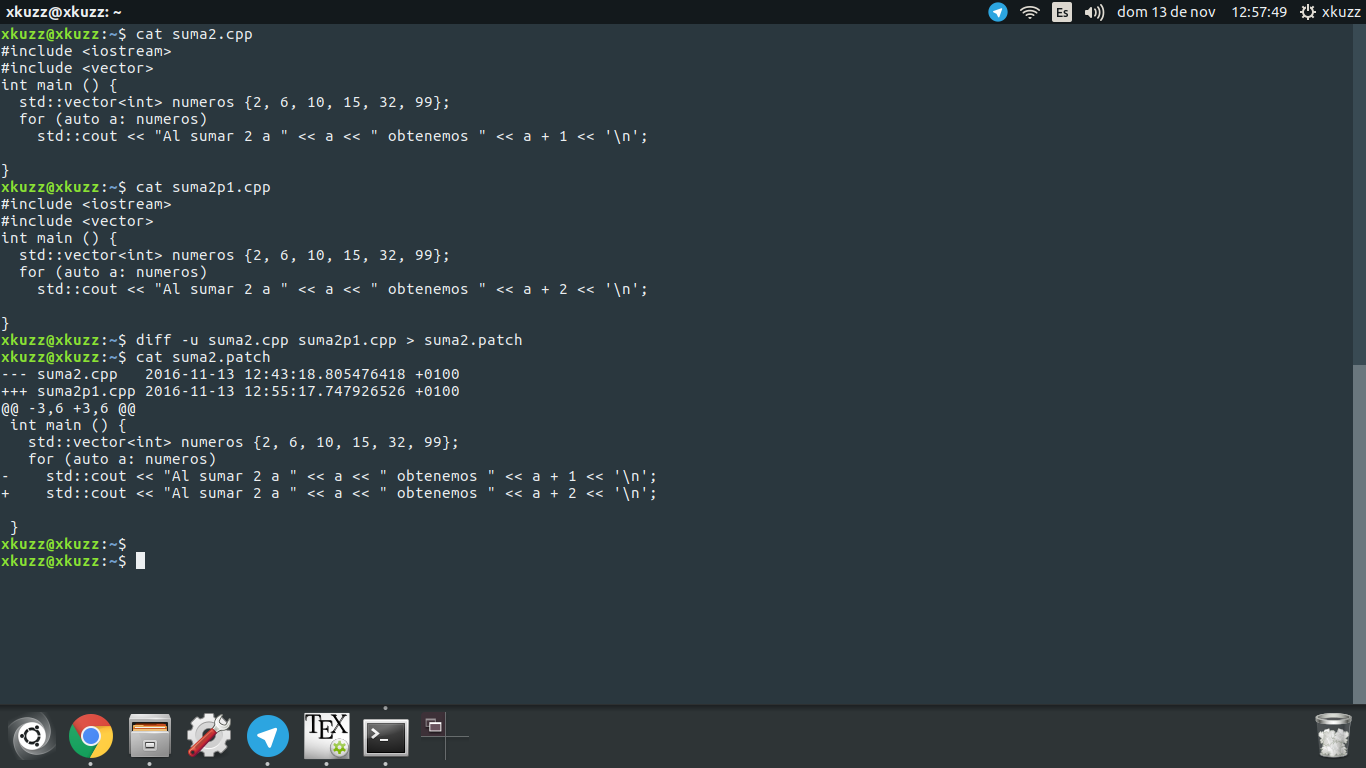
\includegraphics[scale=0.3]{patch1.png}
	\caption{Creamos el patch y vemos su contenido con cat.}
\end{figure}

Tras ver que el programa no funciona correctamente, aplicamos el parche, compilamos y vemos que ahora sí funciona correctamente.

\begin{figure}[H]
	\centering
	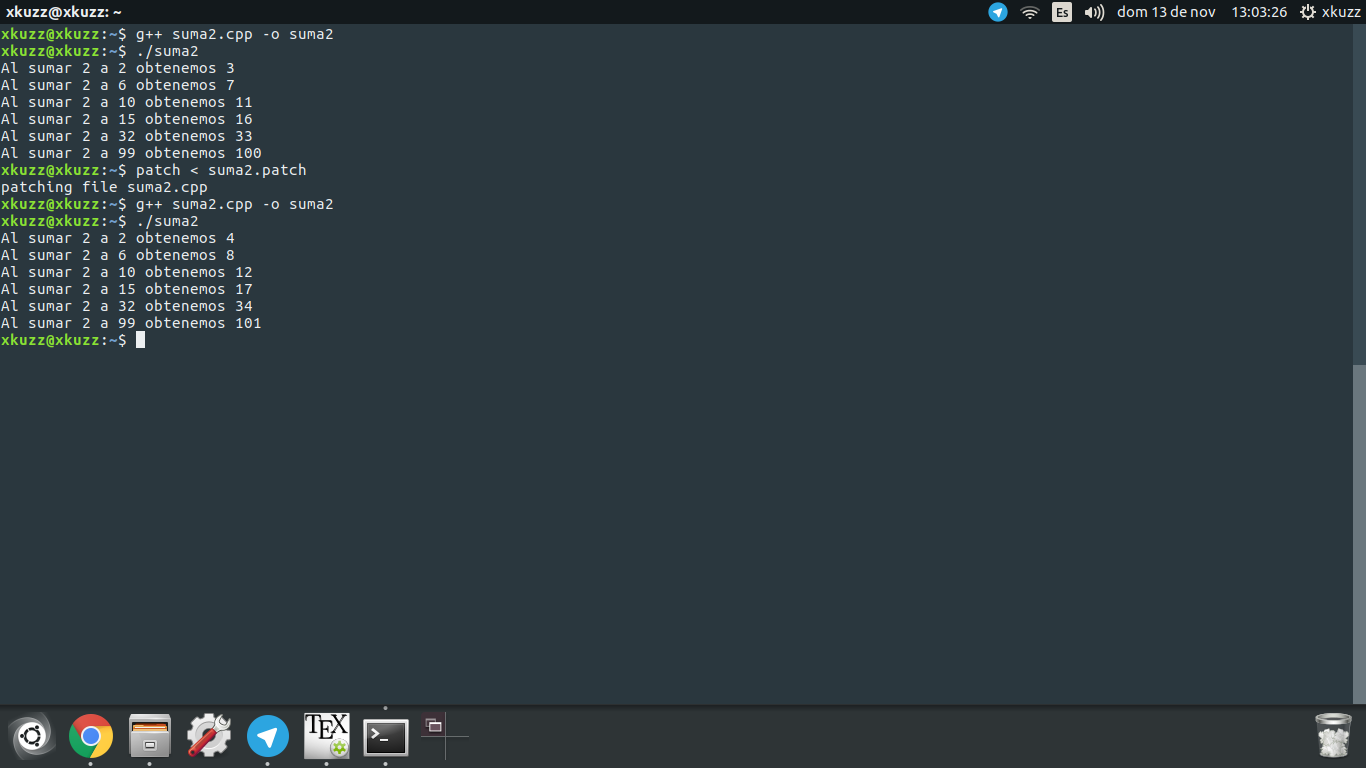
\includegraphics[scale=0.3]{patch2.png}
	\caption{Probamos el programa, aplicamos el patch y volvemos a probar.}
\end{figure}




%----------------------------------------------------------------------------------------
%	Cuestión 12
%----------------------------------------------------------------------------------------
\section{Realice la instalación de webmin y pruebe a modificar algún parámetro de algún servicio. Muestre las capturas de pantalla pertinentes así como el proceso de instalación.}
\subsection{Instalación en Ubuntu Server 14.04}
Desde la página web de webmin \cite{c12a} podemos descargar las versión para sistemas basados en debian. Para ello ejecutamos la siguiente secuencia de comandos, que descargará el paquete a instalar, instalará las dependencias necesarias y, por último, instalará el paquete.

\begin{itemize}
	\item \verb|wget http://prdownloads.sourceforge.net/webadmin/webmin_1.820_all.deb|
	\item \verb|sudo apt install perl libnet-ssleay-perl openssl libauthen-pam-perl| \linebreak 
	      \verb|libpam-runtime libio-pty-perl apt-show-versions python|
	\item \verb|sudo dpkg --install webmin_1.820_all.deb|
\end{itemize}

Tras la instalación nos dice que podemos acceder desde localhost en el puerto 10000, así que para poder acceder desde la máquina anfitriona abrimos el puerto 10000 con el comando \verb|sudo ufw allow 10000|. 

Tras ello podemos acceder con protocolo HTTPS desde nuestro navegador web tras aceptar que, según Google Chrome, el sitio web no es seguro al no proporcionar un certificado inválido. Podemos acceder o con cuenta de root o con la cuenta de cualquier usuario con privilegio sudo y su correspondiente contraseña en el sistema operativo llegando al panel inicial que se muestra en la siguientes figuras.

\begin{figure}[H]
	\centering
	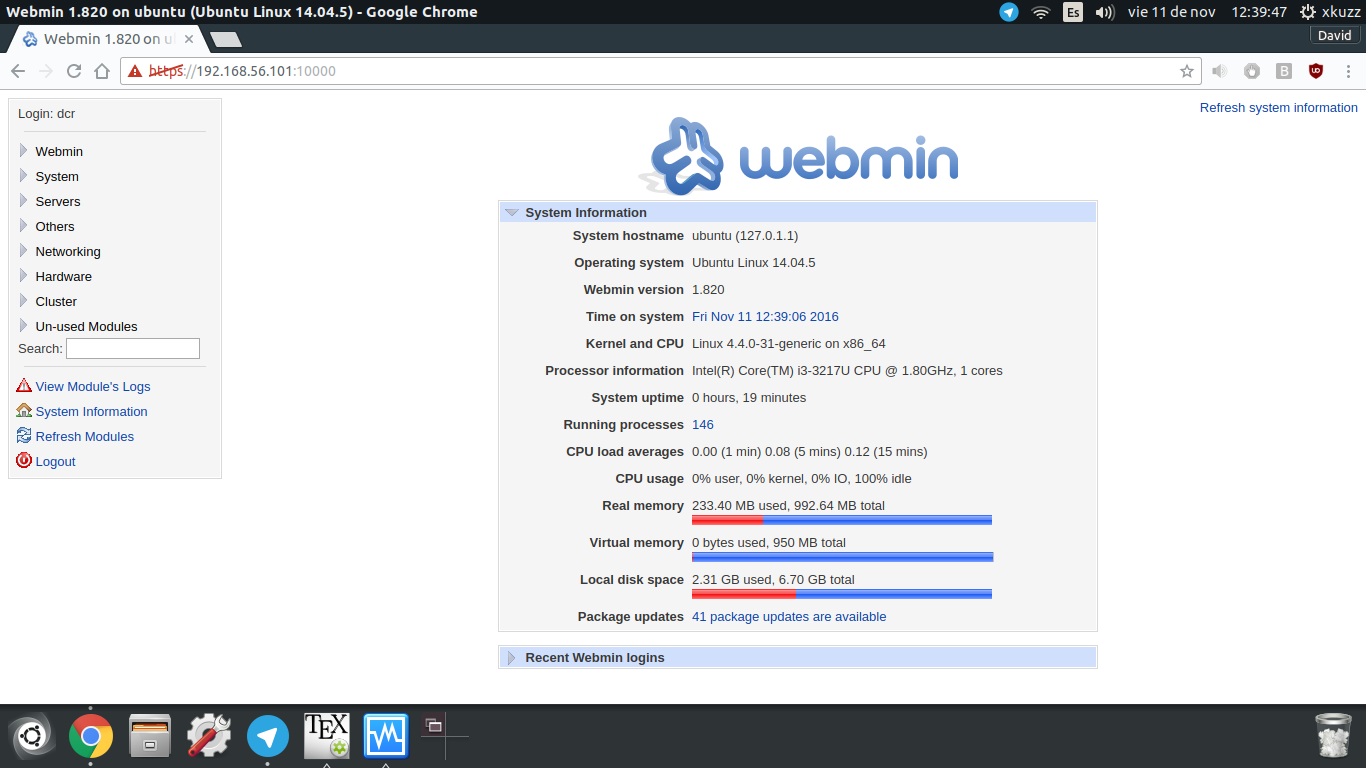
\includegraphics[scale=0.3]{webmin1.png}
	\caption{Panel de webmin (Ubuntu Server 14.04) tras entrar con mi usuario (dcr) y mi contraseña en el sistema.}
\end{figure}

\subsection{Instalación en CentOS 7}
Para instalarlo en CentOS realizamos lo siguiente: \cite{c12a1}
\begin{itemize}
	\item \verb|wget http://prdownloads.sourceforge.net/webadmin/webmin-1.820-1.noarch.rpm|
	\item \verb|yum -y install perl perl-Net-SSLeay openssl perl-IO-Tty|
	\item \verb|rpm -U webmin-1.820-1.noarch.rpm|
\end{itemize}

Por último, al igual que en Ubuntu, debemos abrir el puerto 10000, así que en un terminal escribimos el siguiente comando \verb|sudo firewall-cmd --add-port=10000/tcp| y \verb|sudo firewall-cmd --reload|

\begin{figure}[H]
	\centering
	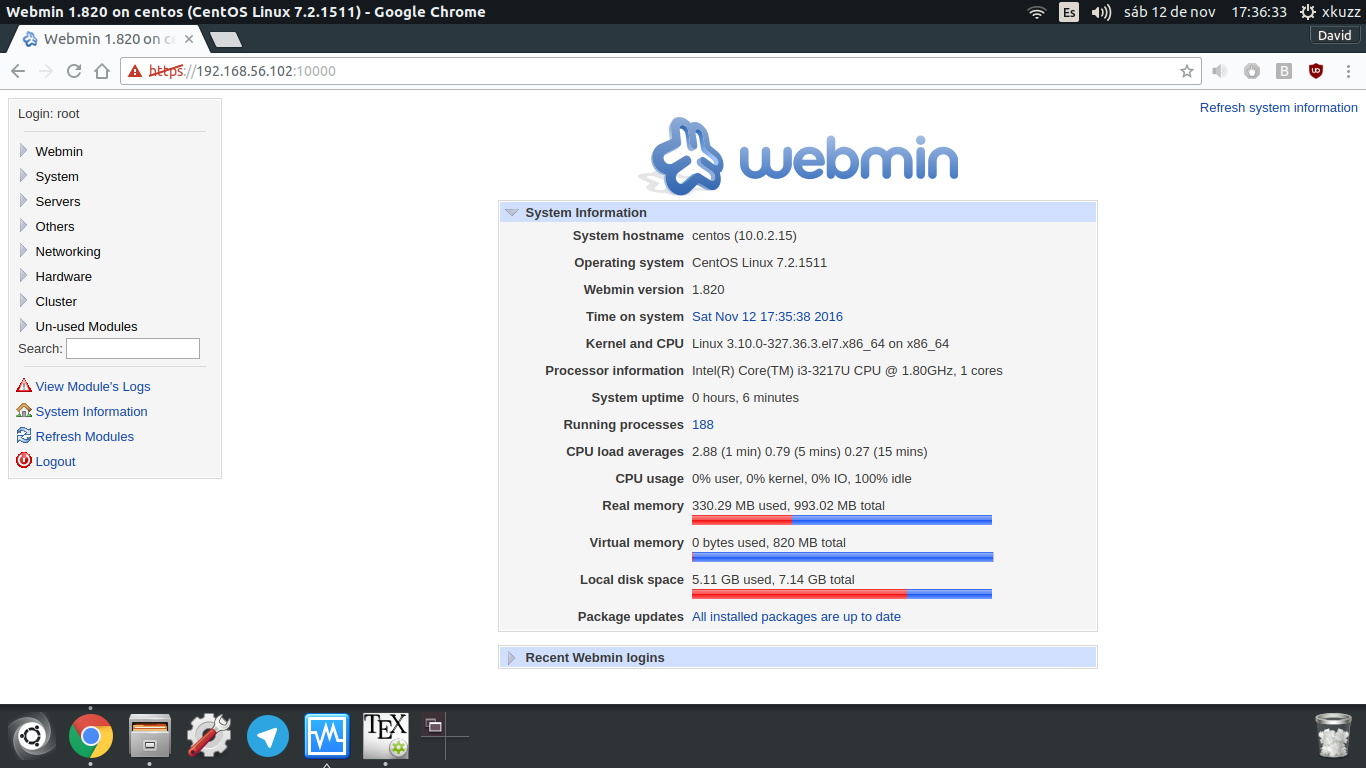
\includegraphics[scale=0.3]{webmin1-c.png}
	\caption{Panel de webmin (CentOS 7) tras entrar con usuario y contraseña del sistema de root.}
\end{figure}

\subsection{Prueba de webmin}
La modificación (realizada en Ubuntu Server) que vamos a hacer es que no se permita acceder al servicio SSH con una contraseña, es decir sólo se permite acceder con una llave. Para ello en el menú lateral seleccionamos Servers > SSH Server > Authentication. En la primera opción (\textit{Allow authentication by password?}) la marcamos a No y pulsamos en Save.

\begin{figure}[H]
	\centering
	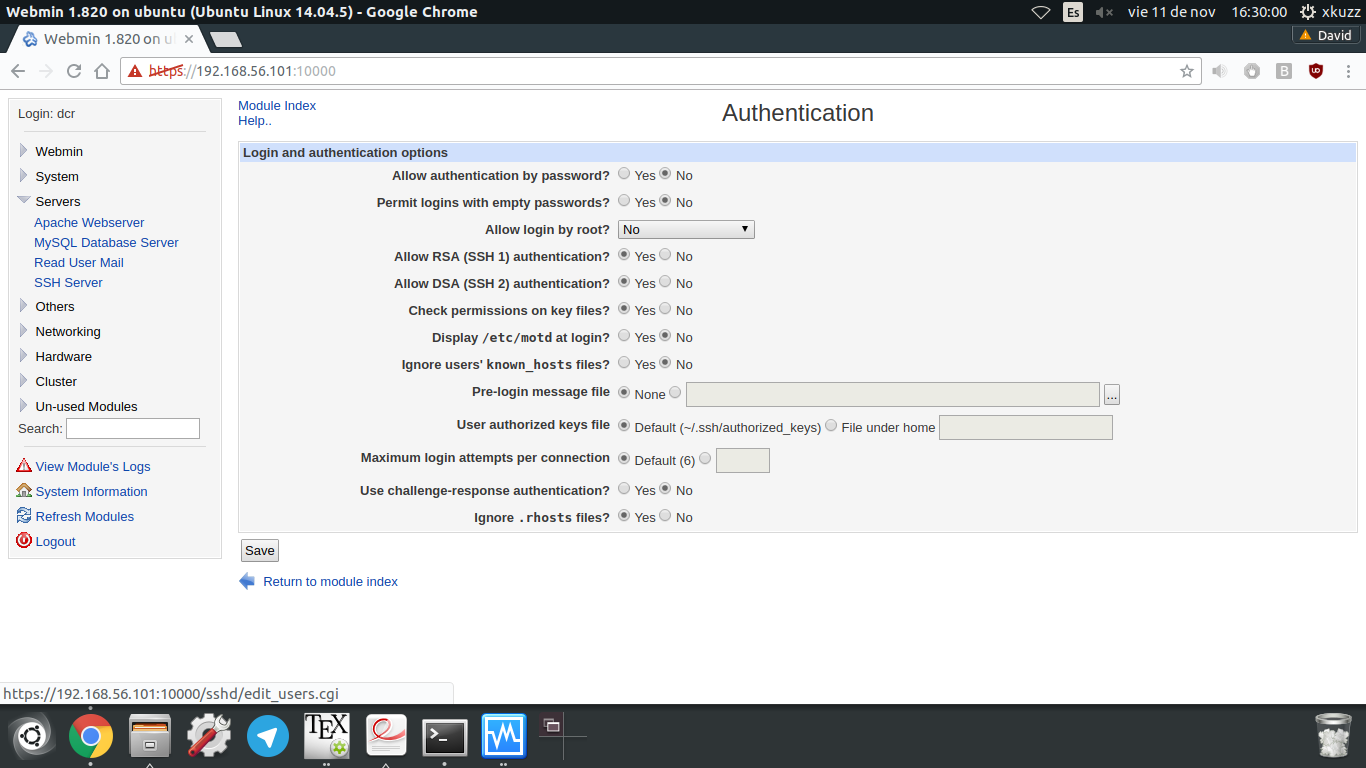
\includegraphics[scale=0.3]{webmin2.png}
	\caption{Opciones de autenticación del servidor SSH desde webmin.}
\end{figure}

Para probar el correcto funcionamiento creo un nuevo usuario dcr2, ya que con dcr tengo creada una llave para acceder, con el script \verb|sudo adduser david| (que nos pedirá contraseña y otros datos opcionales). Una vez creado procedo a procedemos a probar a acceder a SSH, no obstante nos deja entrar.

\begin{figure}[H]
	\centering
	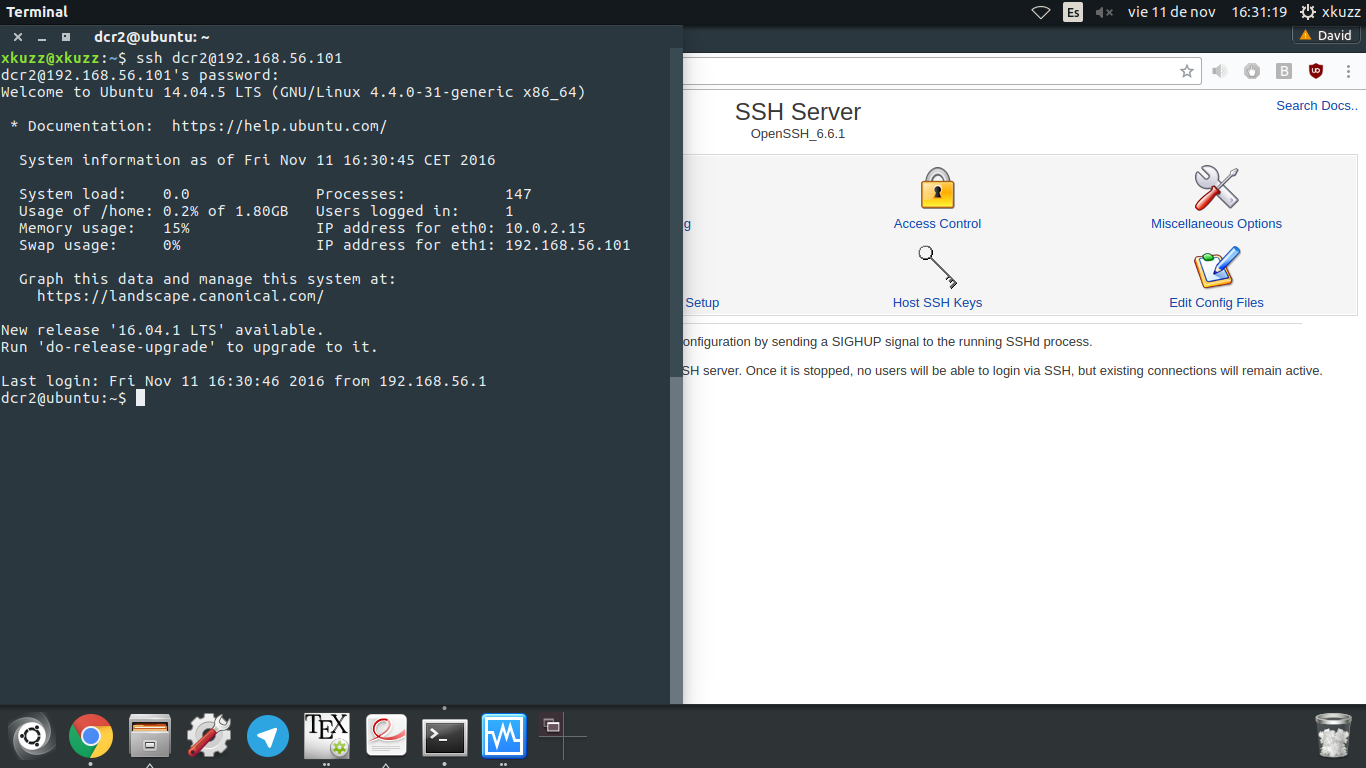
\includegraphics[scale=0.3]{webmin3.png}
	\caption{Accedemos al servicio SSH con la contraseña del nuevo usuario.}
\end{figure}

Para que funcione es necesario pulsar el botón \textit{Apply Changes} y entonces no nos dejará acceder con contraseña.

\begin{figure}[H]
	\centering
	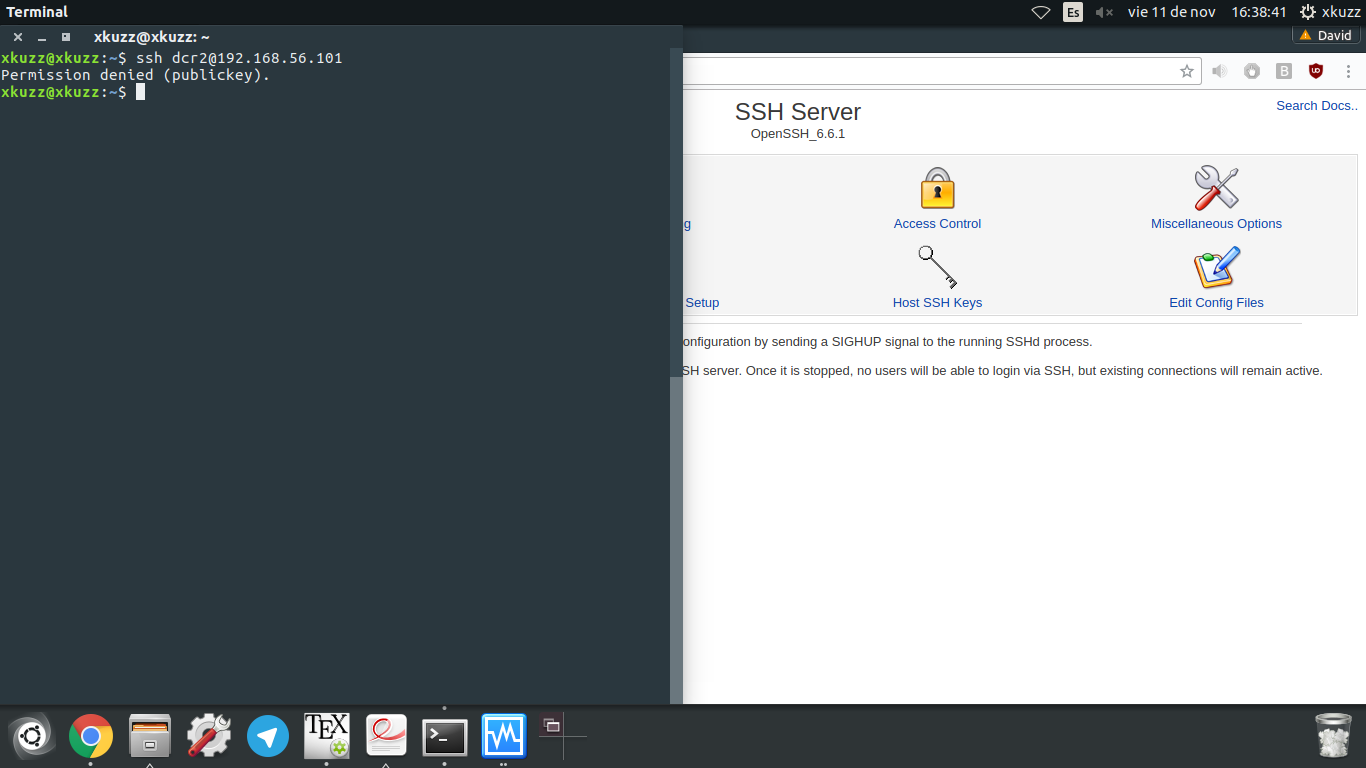
\includegraphics[scale=0.3]{webmin4.png}
	\caption{Se nos niega el acceso tras aplicar los cambios.}
\end{figure}


%----------------------------------------------------------------------------------------
%	Cuestión 13
%----------------------------------------------------------------------------------------
\section{Instale phpMyAdmin, indique cómo lo ha realizado y muestre algunas capturas de pantalla. Configure PHP para poder importar BDs de hasta 25MiB (en vez de los 8 MiB de límite por defecto). Indique cómo ha realizado el proceso y muestre capturas de pantalla.}
\subsection{Instalación en Ubuntu Server 14.04}
Para instalarlo en Ubuntu \cite{c13a} utilizamos el comando (con permisos de administrador) apt install phpmyadmin. Durante el proceso de instalación nos aparecerán dos pantallas: la primera nos permite escoger los servidores web en los que queremos instalar phpMyAdmin (en el que escogeremos apache), y la segunda nos permitirá utilizar una utilidad para configurar la base de datos, marcamos que sí e introducimos la contraseña que root de MySQL.
\linebreak
Anteriormente vimos una imagen de la pantalla de acceso \ref{fig:phpmyadmin} y aquí podemos el panel que entramos una vez iniciamos sesión.
\begin{figure}[H]
	\centering
	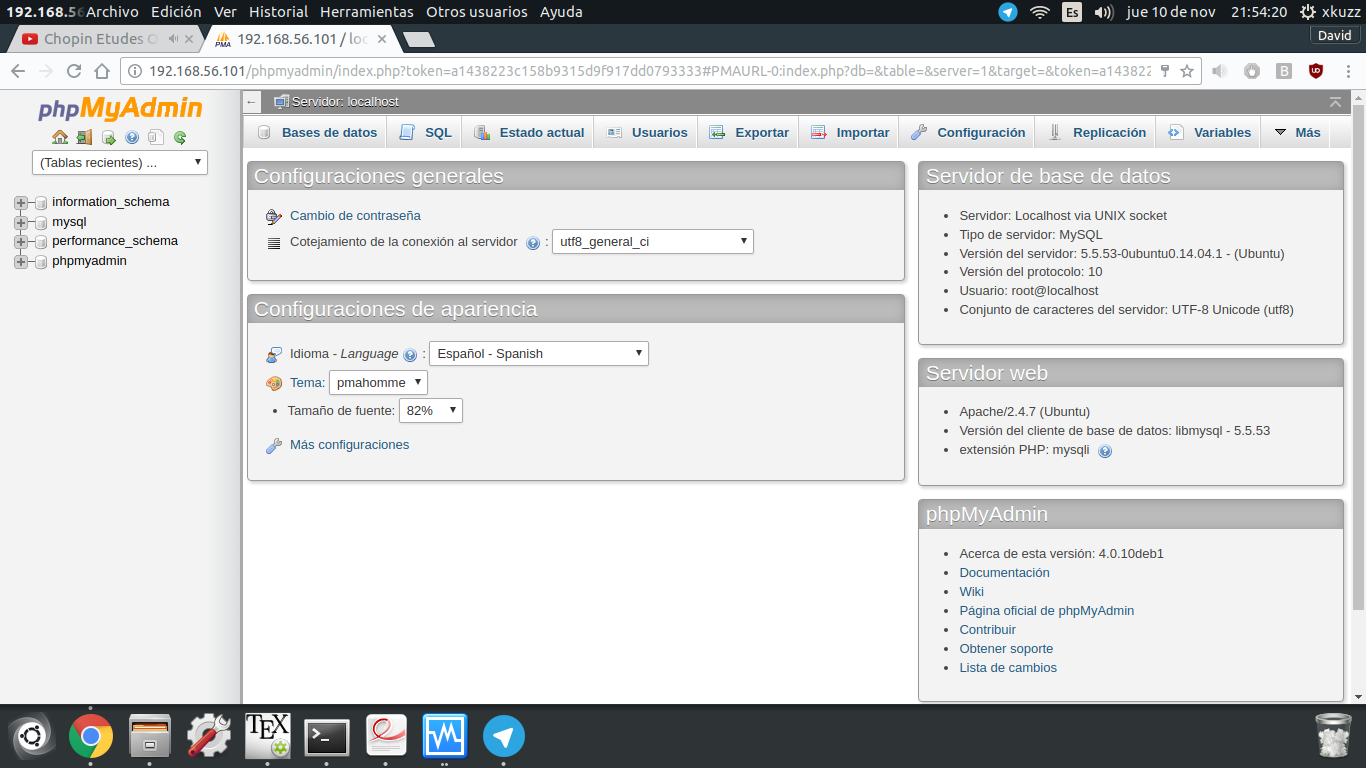
\includegraphics[scale=0.3]{phpmyadmin2.png}
	\caption{Panel de control de phpmyadmin en Ubuntu Server 14.04.}
\end{figure}

\subsection{Instalación en CentOS 7}
No existe repositorio desde el que directamente podamos instalarlo en Centos, así que tal y como dice la documentación de phpMyAdmin \cite{c13a-c}, utilizaremos el repositorio EPEL(Extra Packages for Enterprise Linux) provisto por Fedora, para poder utilizar en Centos sólo debemos usar el comando \verb|sudo yum install epel-release| y tras ello podremos realizar la instalación de phpMyAdmin con el comando \verb|sudo yum install phpmyadmin|.

\begin{figure}[H]
	\centering
	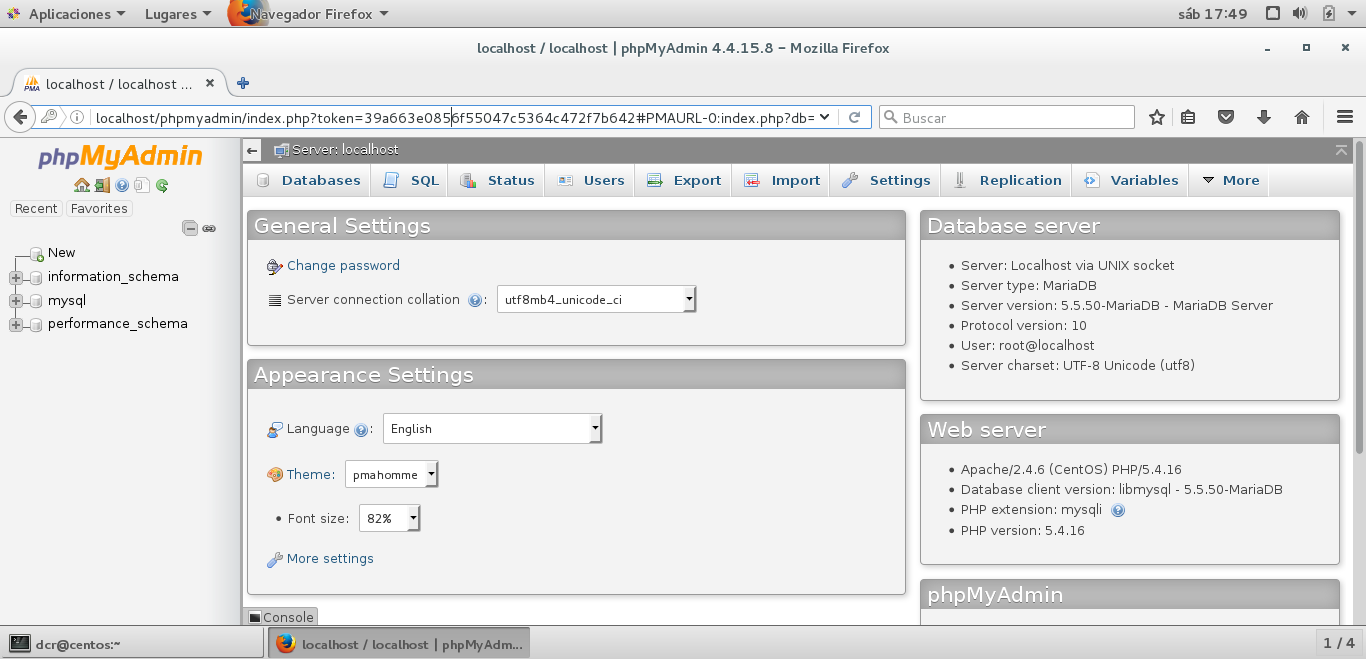
\includegraphics[scale=0.4]{phpmyadmin-c.png}
	\caption{Panel de control de phpmyadmin en Centos 7.}
\end{figure}

\subsection{Configurar PHP para importar BDs de hasta 25 MiB}
Al principio de por sí la configuración inicial de php nos limita las subidas 2 MiB por lo que modificamos la siguiente línea del archivo /etc/php5/apache2/php.ini \verb|max_upload_filesize=25M| (Tamaño máximo de subida de archivo). No obstante, ahora se nos limita a 8 MB (tras reiniciar el servicio de apache) tal y como nos indica el enunciado y como podemos apreciar en la siguiente imagen.
\begin{figure}[H]
	\centering
	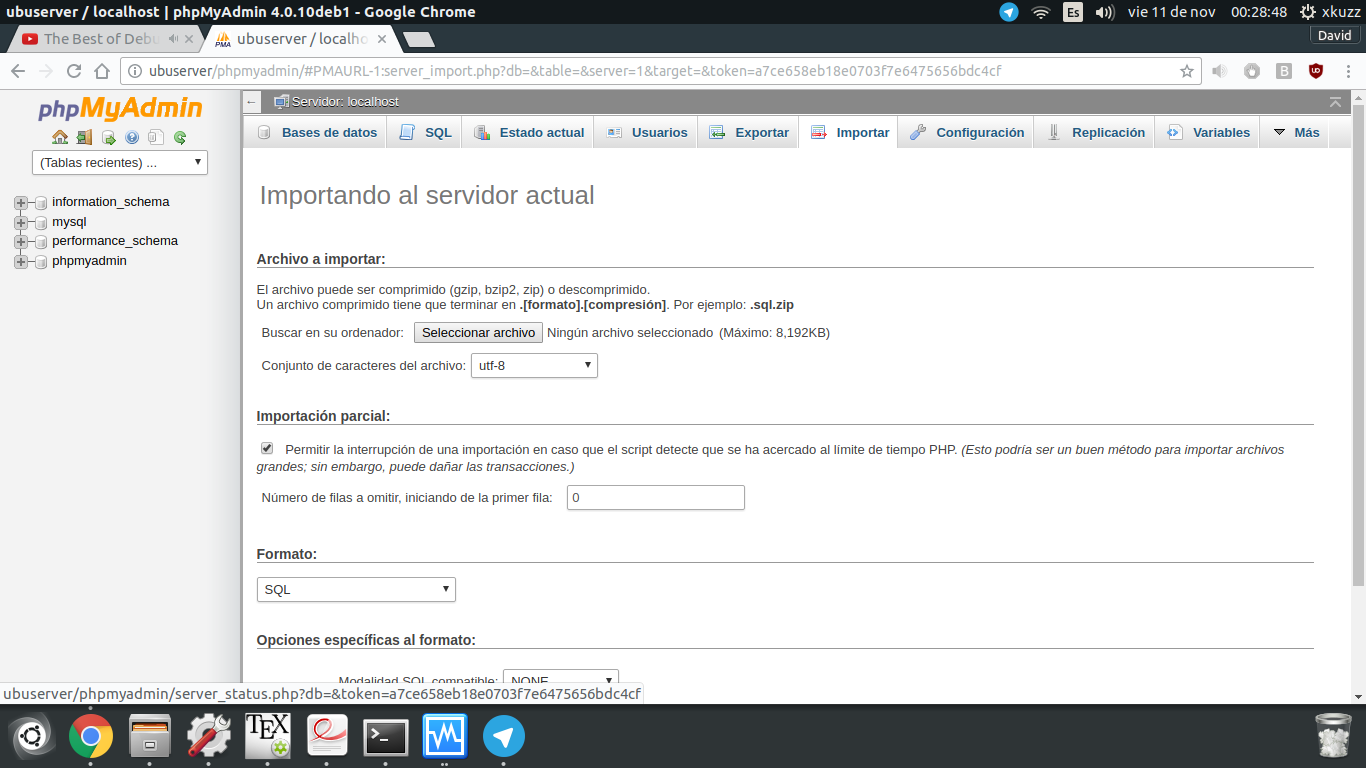
\includegraphics[scale=0.3]{phpmyadmin4.png}
	\caption{Importar con límite de 8 MiB.}
\end{figure}

Para conseguirlo hemos de modificar otro parámetro del mismo archivo \verb|post_max_size=25M|. \cite{c13b}
\begin{figure}[H]
	\centering
	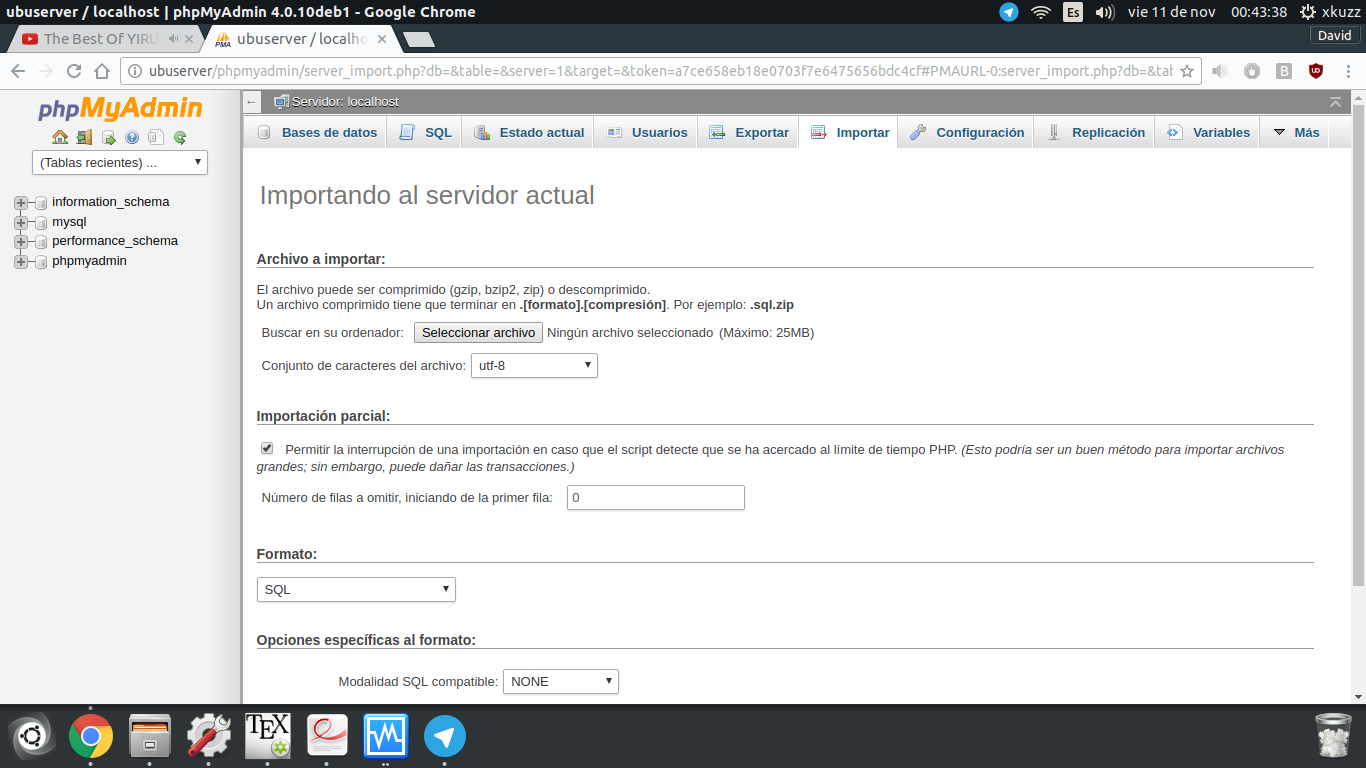
\includegraphics[scale=0.3]{phpmyadmin5.png}
	\caption{Tras modificar ambos parámetros conseguimos la posibilidad de subir un archivo de 25 MB.}
\end{figure}

%----------------------------------------------------------------------------------------
%	Cuestión 14
%----------------------------------------------------------------------------------------
\section{Visite al menos una de las webs de los software DirectAdmin e Ispconfig y pruebe las demos que ofrecen realizando capturas de pantalla y comentando qué está realizando.}

\subsection{Prueba de DirectAdmin}
Tras entrar con los datos de la demo para administradores llegamos al panel de control que vemos en la figura. Podemos diferenciar tres secciones en el centro (Administración del Servidor, Herramientas de Administración y Características Extra). Aparte en el menú superior vemos la posibilidad de un webmail, una contraseña, y a la derecha la información de disco duro y ancho de banda usada, así como información de dominio, usuarios y ``resellers''.

\begin{figure}[H]
	\centering
	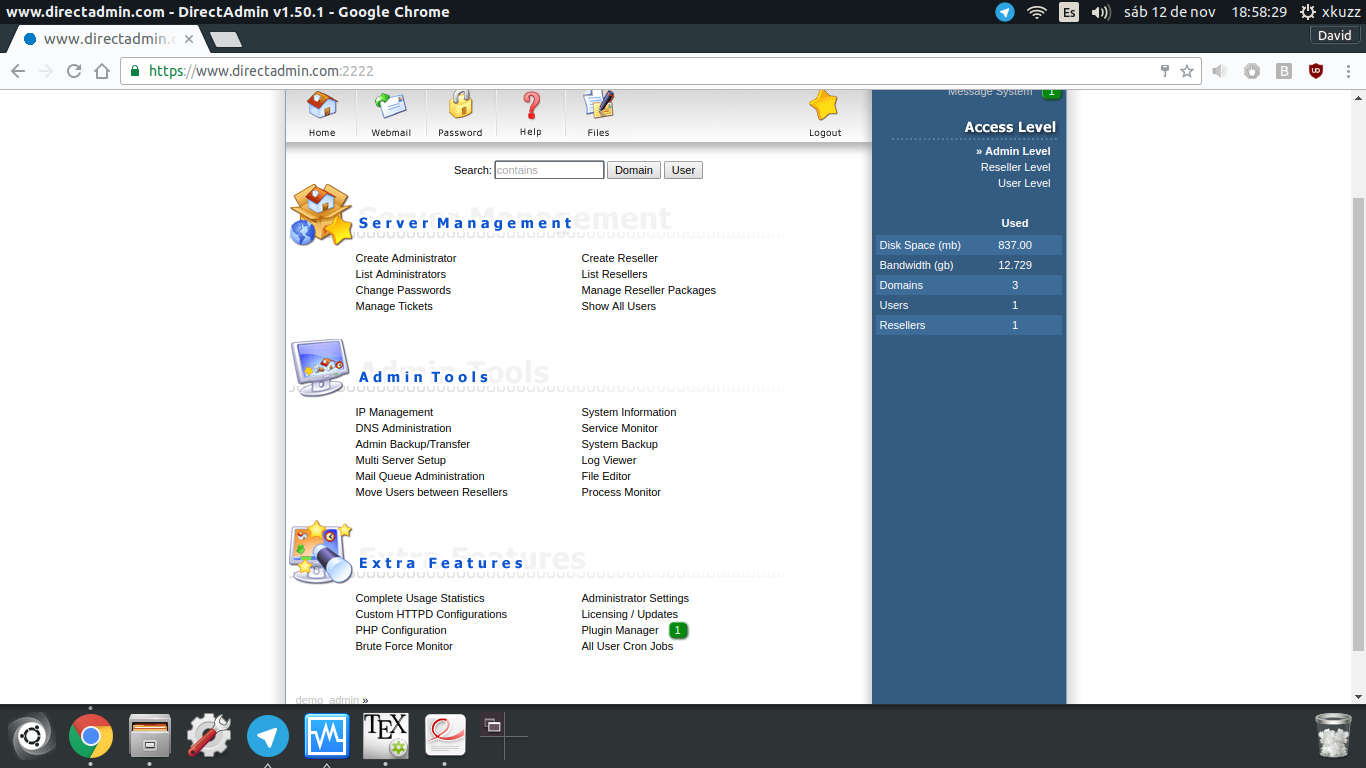
\includegraphics[scale=0.3]{directadmin.png}
	\caption{Panel inicial de la demo de DirectAdmin.}
\end{figure}

Vamos a probar algo de cada sección: En la sección de Administración del Servidor podemos añadir diferentes tipos de usuarios \textit{(Admin, Reseller, User)} y mostrarlos en una lista.
Por ejemplo vamos a ver la lista de los administradores, donde podemos ver características similares a las que veíamos en el menú lateral al inicio pero para cada administrador con la posibilidad de suspender o quitar la suspensión de una cuenta y mandar un mensaje.

\begin{figure}[H]
	\centering
	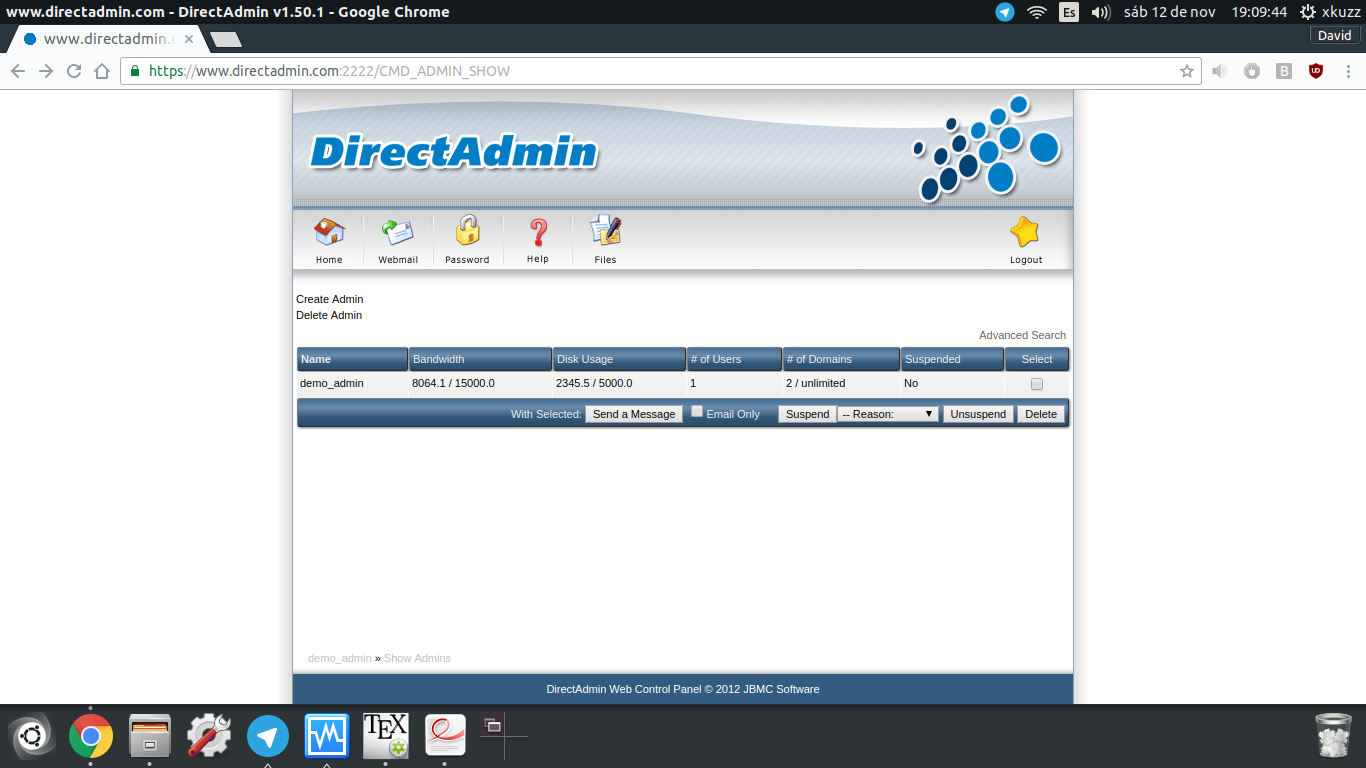
\includegraphics[scale=0.3]{directadmin1.png}
	\caption{Lista de administradores en DirectAdmin,}
\end{figure}

En el panel de Herramientas de Administración, tenemos la mayor parte de opciones, por ejemplo probemos su monitor de procesos (también podemos ver un monitor para servicios). En él podemos ver una estructura similar a la del monitor interactivo de Linux ``top'' y la posibilidad de poner la contraseña de root para mandar señales a dichos procesos.

\begin{figure}[H]
	\centering
	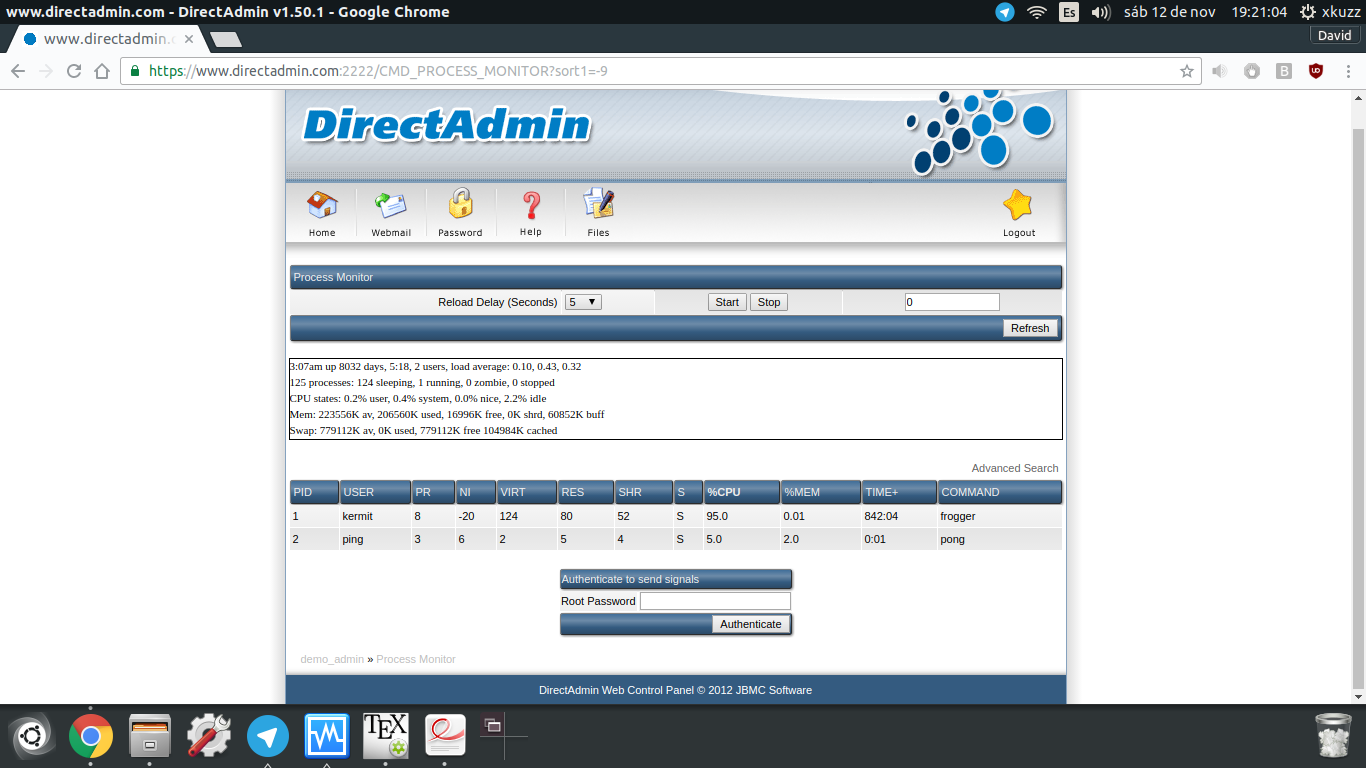
\includegraphics[scale=0.3]{directadmin2.png}
	\caption{Monitor de procesos de DirectAdmin.}
\end{figure}

En ese panel tenemos otras opciones interesantes como ver la información del sistema, administración de IP y DNS, copias de seguridad del servidor, poder ver logs y editar archivos.

En el último panel(Características Extra) tenemos otras opciones como ver Crob Jons, configurar el servidor HTTP, estadísticas completas o un monitor de fuerza bruta. Yo voy a ver la configuración de PHP. En ella simplemente se listan los dominios y su usuario, si tienen activo PHP y si este se encuentra en modo seguro. Desde este panel el administrador puede configurar los valores por defecto y seleccionar dominios y modificar estos valores para ellos.

\begin{figure}[H]
	\centering
	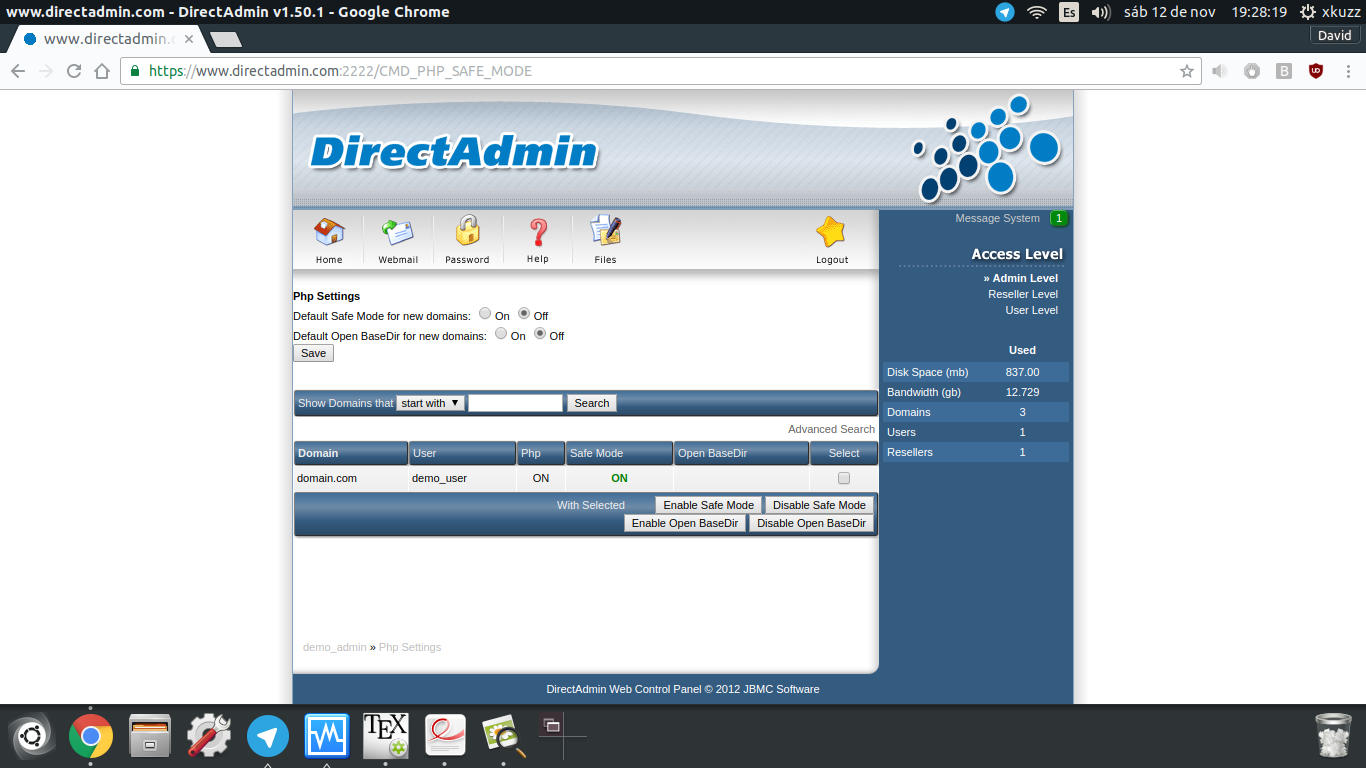
\includegraphics[scale=0.3]{directadmin3.png}
	\caption{Configuración de PHP de DirectAdmin.}
\end{figure}

De las opciones superiores vamos a meternos en archivos. En esta podemos ver y movernos por los directorios, modificar permisos así como su creador y mover, copiar y borrar archivos y directorios.

\begin{figure}[H]
	\centering
	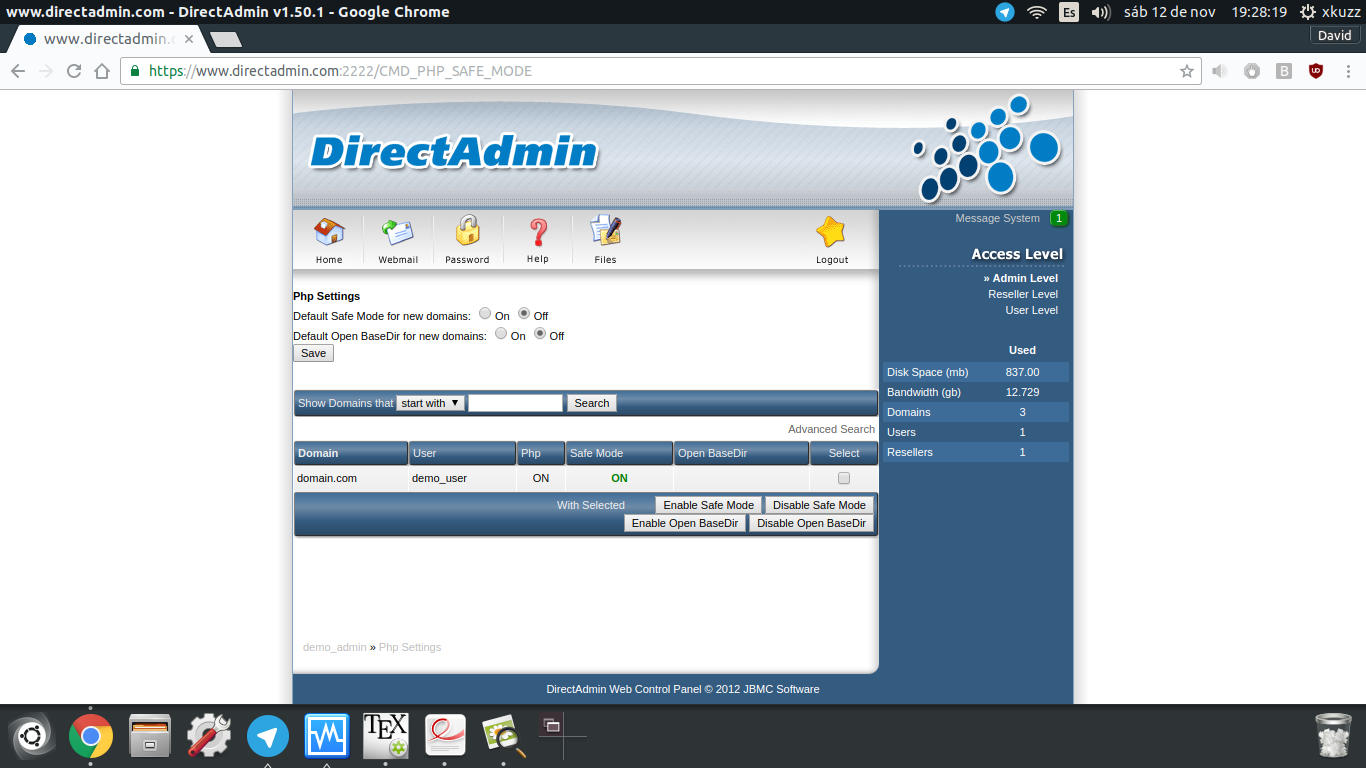
\includegraphics[scale=0.3]{directadmin3.png}
	\caption{Archivos de DirectAdmin.}
\end{figure}


%----------------------------------------------------------------------------------------
%	Cuestión 15
%----------------------------------------------------------------------------------------
\section{Ejecute los ejemplos de find, grep. Escriba el script que haga uso de sed para cambiar la configuración de ssh y reiniciar el servicio. Muestre un ejemplo de uso para awk.}

\subsection{Ejecute los ejemplos de find, grep.}
\begin{figure}[H]
	\centering
	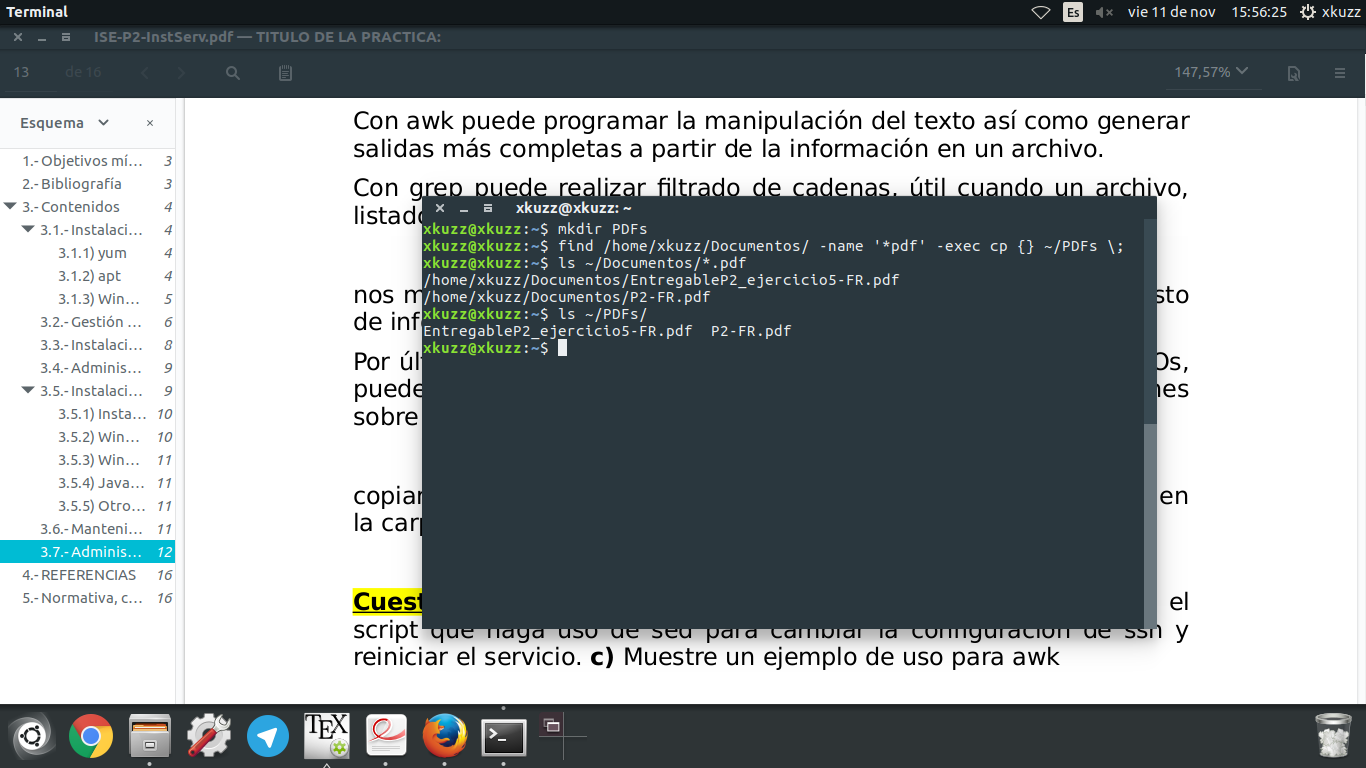
\includegraphics[scale=0.3]{find.png}
	\caption{find copia los dos archivos PDF encontrados a la carpeta.}
\end{figure}

\textit{find} nos permite encontrar elementos en la jerarquía de archivos del sistema Linux. En el ejemplo propuesto se buscan archivos que acaben en pdf (-name '*PDF') y nos permite ejecutar (-exec) un comando que se llama cada vez que se encuentra un archivo (en el ejemplo copiarlos a un directorio llamado PDFs). El nombre de cada uno de esos archivos encontrados se escribe dentro del comando ejecutado por exec como \verb|{}|. \cite{c15a}

\begin{figure}[H]
	\centering
	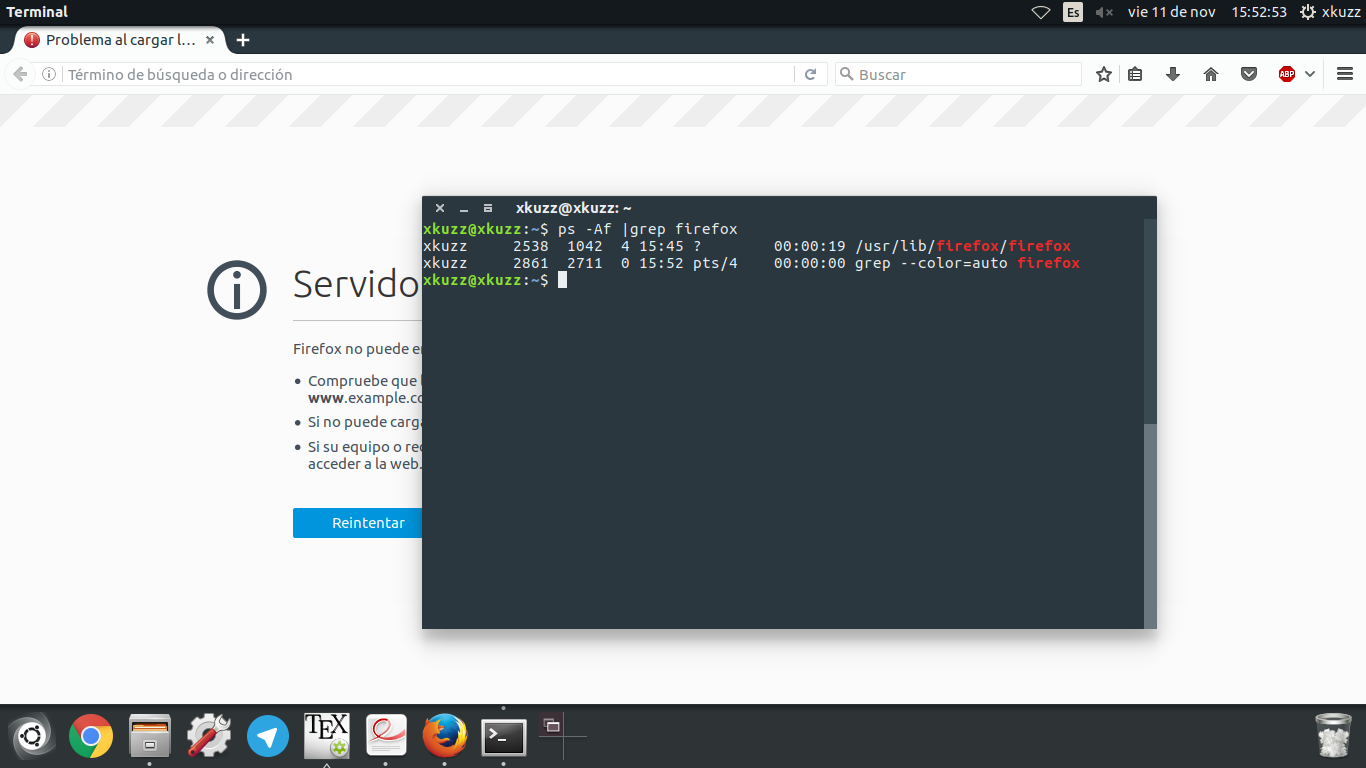
\includegraphics[scale=0.3]{grep.png}
	\caption{grep filtra el proceso del navegador Firefox de la lista de procesos.}
\end{figure}

\textit{grep} busca en un texto una línea que contenga el patrón que se nos ha dado así en el ejemplo podemos filtrar la línea que hace referencia al proceso de Firefox del resto de líneas que no nos interesan.\cite{c15a2}

\subsection{Escriba el script que haga uso de sed para cambiar la configuración de ssh y reiniciar el servicio.}
\textit{sed} nos permite realizar cambios sobre un archivo con el parámetro -i. La opción \verb|\c| además nos permite que solo las cadenas que se correspondan al patrón proporcionado antes del mismo se modifiquen por el patrón proporcionado a continuación. \cite{c15b}

Puesto que el parámetro que queremos modificar de la configuración de SSH es PasswordAuthentication \cite{c7b}, que nos permite determinar si se puede acceder con la contraseña de usuario o no (sólo se permite acceder con una llave) los comandos a utilizar para cambiar el archivo de configuración serían los siguientes:

\begin{itemize}
	\item \textbf{Para activar} \begin{verbatim}
	sed -i '/PasswordAuthentication no/c\PasswordAuthentication yes'
	 /etc/ssh/sshd_config
	\end{verbatim}
	\item \textbf{Para desactivar} \begin{verbatim}
	sed -i '/PasswordAuthentication yes/c\PasswordAuthentication no'
	 /etc/ssh/sshd_config
	 \end{verbatim}
\end{itemize}
El script sería el siguiente:

\begin{verbatim}
if [ $# -eq 1 ] 
then
  if [ "$1" = "on" ]
  then
    sed -i '/PasswordAuthentication no/c\PasswordAuthentication yes' /etc/ssh/sshd_config
    service ssh restart
    echo "Acceso con contraseña activado."
  elif [ "$1" = "off" ]
  then   
    sed -i '/PasswordAuthentication yes/c\PasswordAuthentication no' /etc/ssh/sshd_config
    service ssh restart
    echo "Acceso con contraseña desactivado."
  else
    echo "Uso correcto: sshpass.sh [on|off]"
  fi
else
  echo "Uso correcto: sshpass.sh [on|off]"
fi
\end{verbatim}


Probemos con un usuario que no tenga llave que el script funciona correctamente.

\begin{figure}[H]
	\centering
	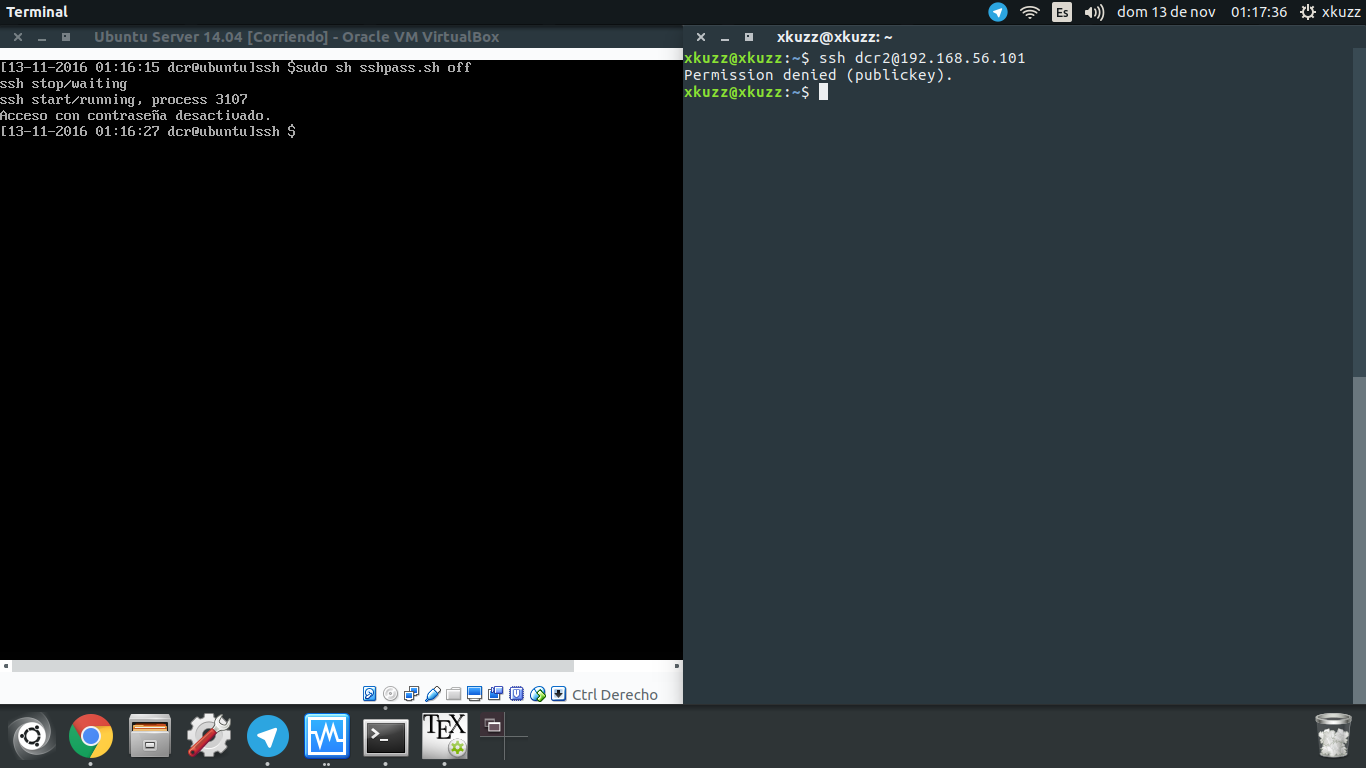
\includegraphics[scale=0.3]{shoff.png}
	\caption{Tras utilizar el script bash para no permitir contraseña se nos deniega el acceso.}
\end{figure}

\begin{figure}[H]
	\centering
	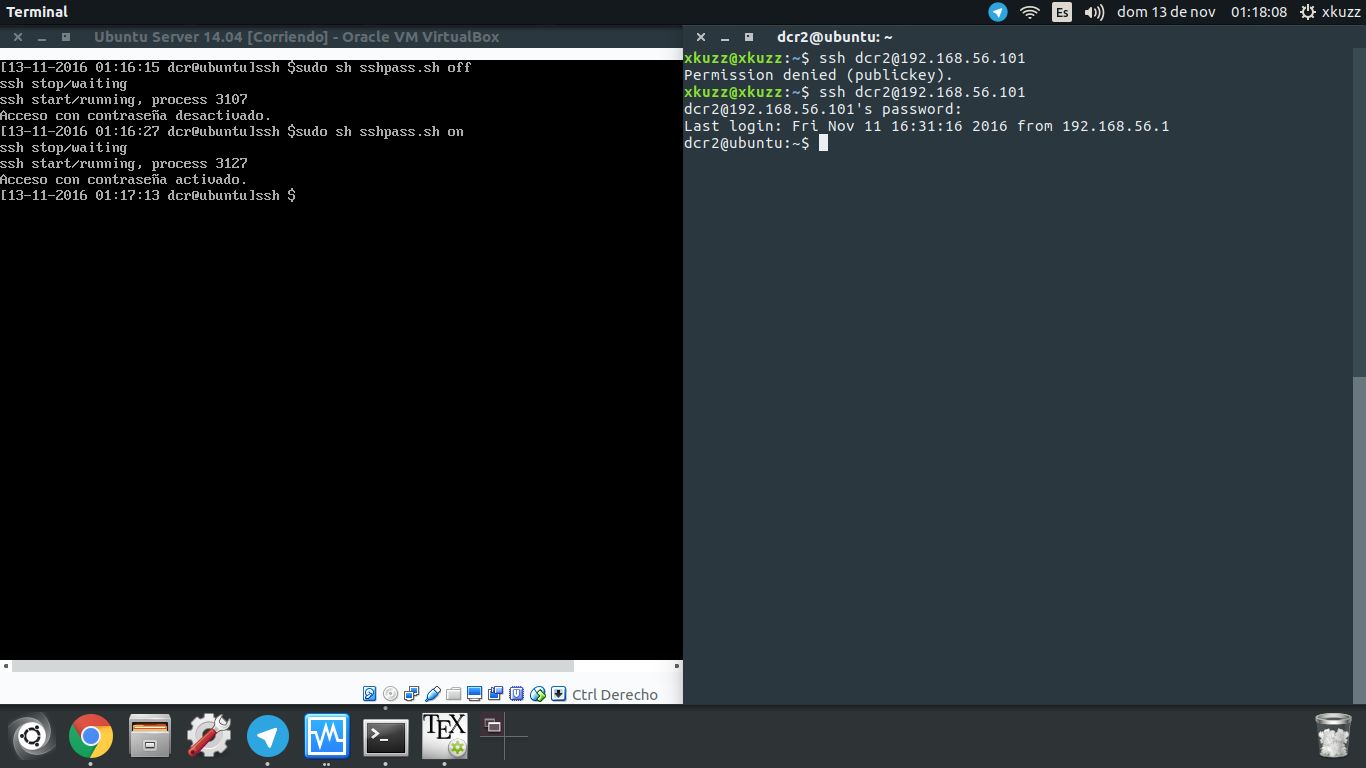
\includegraphics[scale=0.3]{shon.png}
	\caption{Tras utilizar el script bash poder usar contraseña podemos acceder.}
\end{figure}

\subsection{Muestre un ejemplo de uso para awk.}
\textit{awk} \cite{c15c} nos puede servir para filtrar datos de un archivo de texto, entre otros, ya que se trata de un lenguaje de programación de texto y escaneo de patrones. Supongamos que tenemos una tabla como la mostrada en la figura. Imaginemos que nos interesan sólo los valores B, D y comentario de las filas que tienen comentarios no más largos de 12 caracteres. Con awk podemos utilizar la función length para saber la longitud de algo y podemos separar la tabla en columnas accediendo con \verb|$1, $2, ..., $n| y con la función print mostrarlo por pantalla.

\begin{figure}[H]
	\centering
	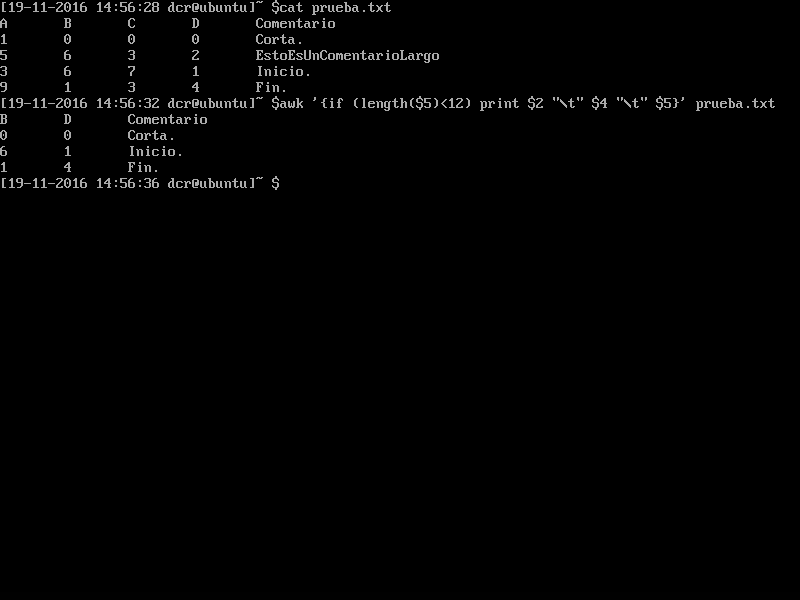
\includegraphics[scale=0.4]{awk.png}
	\caption{Filtramos datos del archivo mostrado usando awk.}
\end{figure}

%----------------------------------------------------------------------------------------
%	Cuestión 16
%----------------------------------------------------------------------------------------
\section{Escriba el script para cambiar el acceso a ssh usando PHP o Python.}
Gracias al método call de la clase subprocess \cite{c16} podemos llamar fácilmente a el comando sed, por tanto,
el script en Python sería el siguiente:
\begin{verbatim}
import os
import subprocess
import sys

def main(argv):
  if os.getuid() != 0:
    print 'El script necesita permisos de administrador'
    sys.exit(-1)

  if len(sys.argv) != 2:
    print 'Uso correcto: sudo python sshpass.py on|off'
    sys.exit(-2)

  opciones = ['on', 'off']
  opcion = argv[0].lower()

  if opcion not in opciones:
    print 'Uso correcto: sudo python sshpass.py on|off'
    sys.exit(-3) 

  if opcion == opciones[1]:
    subprocess.call(['sed', '-i', 
    '/PasswordAuthentication yes/c\\PasswordAuthentication no', '/etc/ssh/sshd_config'])
  else:
    subprocess.call(['sed', '-i', 
    '/PasswordAuthentication no/c\\PasswordAuthentication yes', '/etc/ssh/sshd_config'])
  subprocess.call(['service', 'ssh', 'restart'])
  sys.exit(0)

if __name__ == "__main__":
   main(sys.argv[1:])
\end{verbatim}

Probemos con un usuario que no tenga llave que el script funciona correctamente.

\begin{figure}[H]
	\centering
	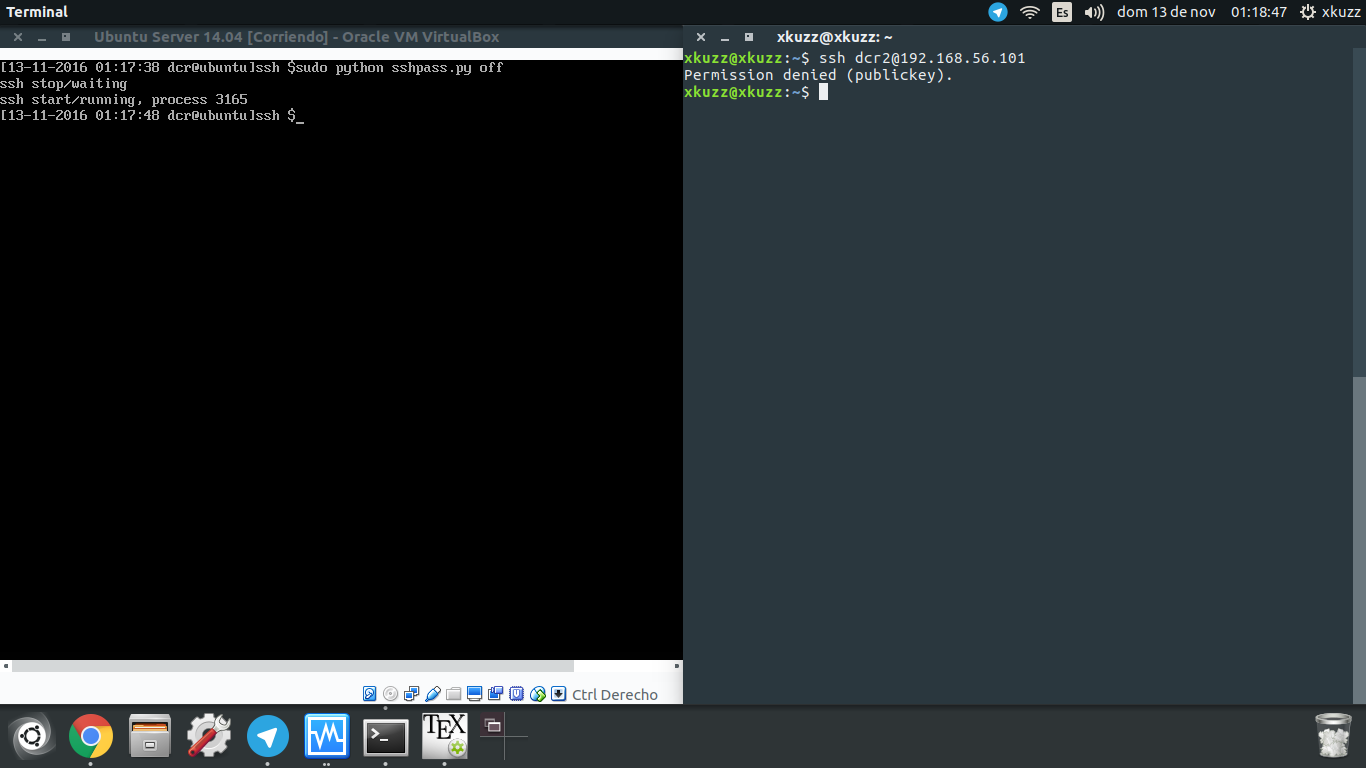
\includegraphics[scale=0.3]{pyoff.png}
	\caption{Tras utilizar el script en Python para no permitir contraseña se nos deniega el acceso.}
\end{figure}

\begin{figure}[H]
	\centering
	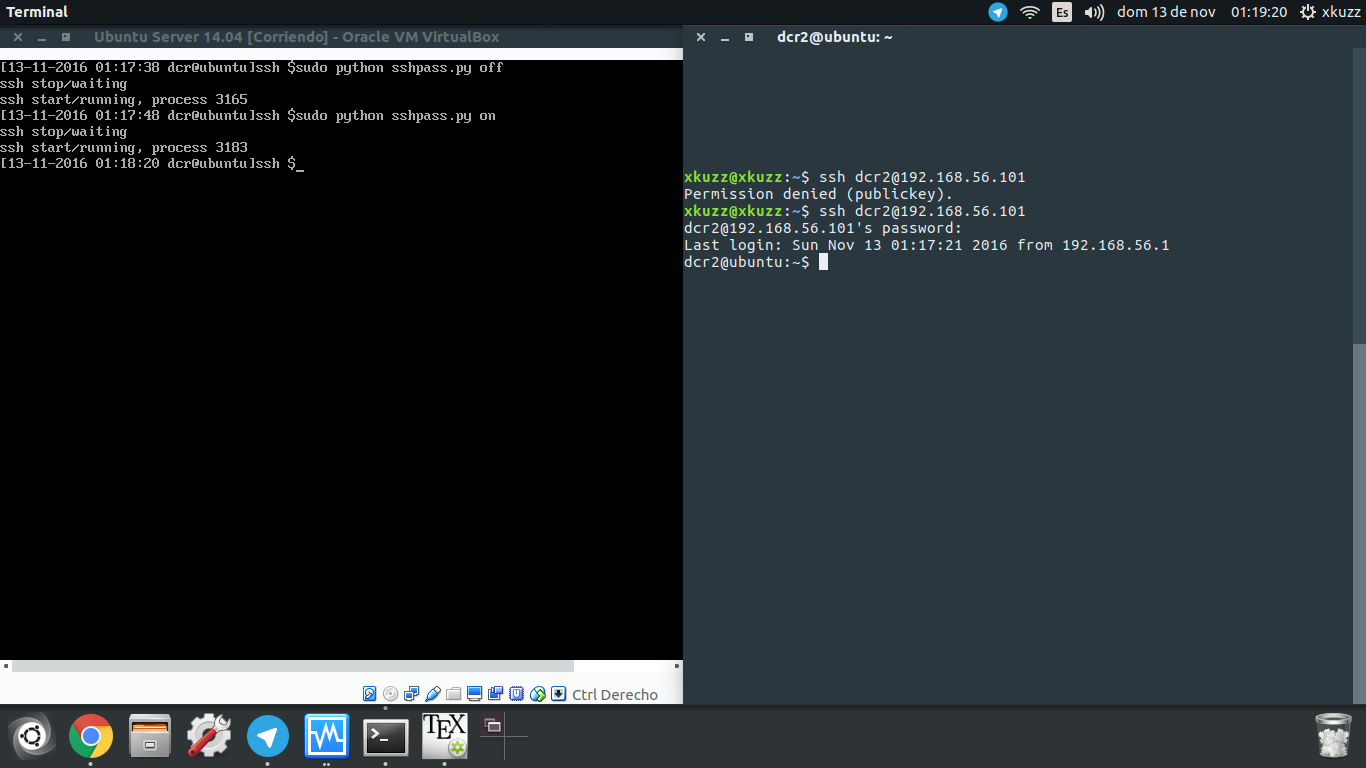
\includegraphics[scale=0.3]{pyon.png}
	\caption{Tras utilizar el script en Python permitir usar contraseña podemos acceder.}
\end{figure}

%----------------------------------------------------------------------------------------
%	Cuestión 17
%----------------------------------------------------------------------------------------
\section{Abra una consola de Powershell y pruebe a parar un programa en ejecución (p.ej), realice capturas de pantalla y comente lo que muestra.}
Por ejemplo vamos a parar la aplicación del GUI ``Administración del Servidor'' que corresponde al proceso ``ServerManager''. Para ello utilizamos el comando \verb|Stop-Process -Name ServerManager| \cite{c17}

Para deducirlo hemos mirado la lista de procesos con el comando \verb|Get-Process| antes y después de la ejecución de la aplicación. En la siguiente captura podemos ver la lista de procesos activos.

\begin{figure}[H]
	\centering
	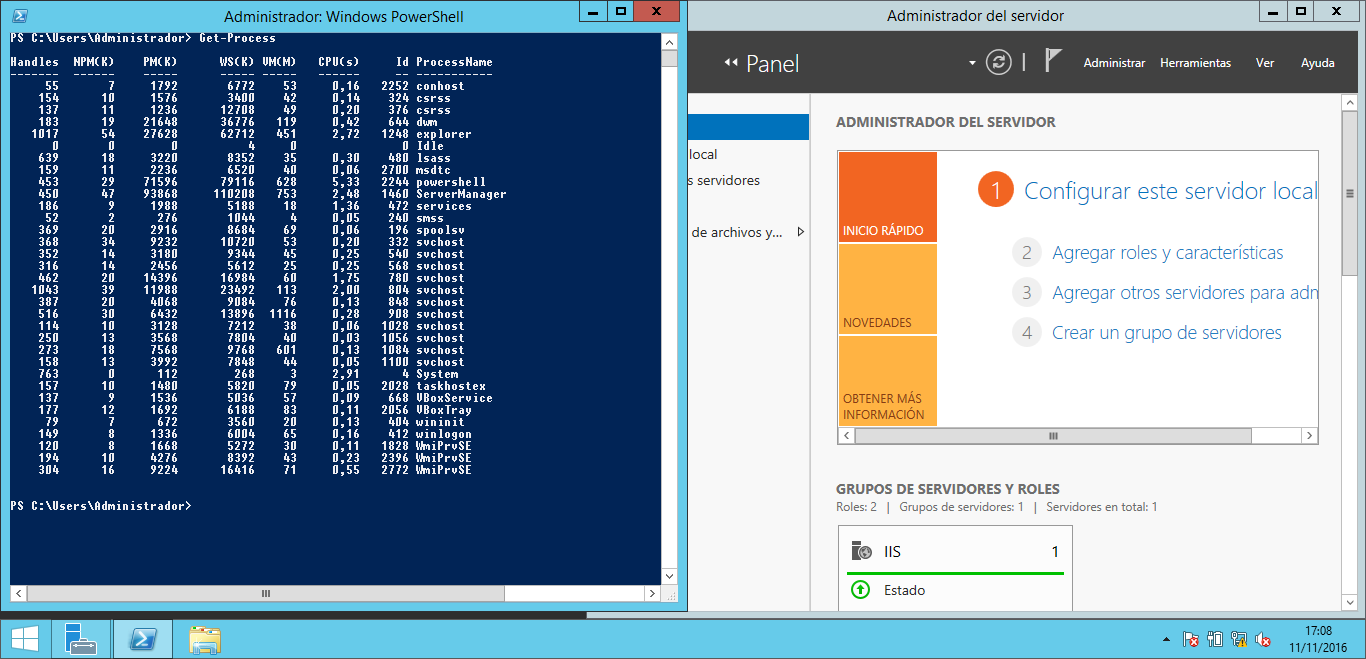
\includegraphics[scale=0.4]{pwshell1.png}
	\caption{Lista de procesos activos desde PowerShell.}
\end{figure}

\begin{figure}[H]
	\centering
	\includegraphics[scale=0.4]{pwshell2.png}
	\caption{Paramos el proceso y probamos a pararlo si no está abierto.}
\end{figure}

Como podemos ver en la imagen anterior si el proceso es parado correctamente no da ningún resultado. En caso contrario, es decir, el proceso no se encuentra ejecutándose tal y como nos indica el mensaje proporcionado en color rojo.
%----------------------------------------------------------------------------------------
%	Bibliografía
%----------------------------------------------------------------------------------------
\bibliography{citas} %archivo citas.bib que contiene las entradas 
\bibliographystyle{ieeetr} % hay varias formas de citar
\end{flushleft}
\end{document}
